\documentclass[12pt]{report}
\usepackage[utf8]{inputenc}
\usepackage{graphicx}
\usepackage{amsmath, amssymb}
\usepackage{geometry}
\usepackage{fancyhdr}
\usepackage{hyperref}
\usepackage{caption} 
\usepackage{float}
\usepackage{listings}
\usepackage{tocbibind} 
\usepackage{titlesec}
\usepackage{booktabs}
\usepackage{array}    
\usepackage{url}

\geometry{a4paper, top=1in, bottom=1in, right=1in, left=1in}
\hypersetup{
    colorlinks=true,
    linkcolor=blue,
    filecolor=magenta,      
    urlcolor=cyan,
}

\renewcommand{\bibname}{References}

% Header customization
\pagestyle{fancy}
\fancyhf{} % Clears any existing header/footer
\fancyhead[L]{\leftmark} % Displays subsection title
\fancyhead[R]{\thepage} % Displays page number on the right
\renewcommand{\headrulewidth}{0.4pt} % Adds a line under the header
\setlength{\headheight}{15pt}

\begin{document}

% Title Page
\begin{titlepage}
    \thispagestyle{empty}
    \centering
    
\includegraphics[width=0.25\textwidth]{asu_logo.png} \hfill
    
\includegraphics[width=0.22\textwidth]{eng_logo.png}
    \vspace{2.5cm}
    
    \LARGE \textbf{FPGA-Based Hardware Acceleration of Numerical Theoretic Transform with RISC-V ISA Customization} \\
    \vspace{0.5cm}
    %{\large \textit{FPGA-Based Hardware Acceleration of NTT with RISC-V ISA Customization}}

    \vspace{1.5cm}

    \large
    Abanoub Emad Hanna \\ \vspace{0.35cm}
    Abdelrhman Emad Fathy \\ \vspace{0.35cm}
    Ahmed Nader Ahmed \\ \vspace{0.35cm}
    Mahmoud Mohamed Soliman \\ \vspace{0.35cm}
    Omar Mahmoud Gabr \\ \vspace{0.35cm}
    Omar Mohamed Afifi
    \vspace{1.5cm}
    
    \textbf{Supervisors: Dr. Hesham Omran \& Dr. Hossam Hassan}
    \vspace{1.5cm}

    Graduation Project Thesis \\
    Electronics and Electrical Communication Engineering \\
    Faculty of Engineering, Ain Shams University \\

\end{titlepage}

\newpage

\section*{Acknowledgements}

We would like to express our deepest gratitude to Dr. Hossam Hassan and Dr. Hesham Omran for their invaluable supervision and guidance throughout our graduation project. Their expertise, patience, and dedication have been instrumental in the successful completion of our work. \\
We would like to acknowledge the support and contributions of all our friends,
colleagues, and family members who have stood by us throughout this project. Their
encouragement, understanding, and patience have been instrumental in keeping us
motivated and focused. We extend our heartfelt appreciation to all those who have
supported us in various ways, and we are truly grateful for their contributions.
The collective contributions have not only made our project possible but also provided
us with a rich learning experience that we will carry forward into our future endeavors. \\
Thank you all!

\newpage

\section*{Abstract}

This thesis presents a hardware accelerator for the Number Theoretic Transform (NTT), a key operation in post-quantum cryptography, integrated with a RISC-V open-source GPU to enhance computational efficiency. The accelerator leverages parallelism and custom hardware design to reduce computation time and energy consumption, addressing the growing demands of real-time cryptographic workloads. \\ \\
A comprehensive evaluation of the NTT accelerator is conducted, focusing on metrics such as latency, throughput, and resource utilization. Experimental simulations and synthesis results demonstrate significant improvements over software-only and traditional hardware implementations. The pipelined and parameterized design highlights the trade-offs between computation speed and resource efficiency, offering a scalable solution for cryptographic applications. \\ \\
The study also explores the integration of the NTT accelerator into a RISC-V-based GPGPU architecture, utilizing SIMT (Single Instruction, Multiple Threads) execution for parallel processing. Custom instructions and optimized memory access patterns are implemented to maximize data throughput and computational efficiency. Additionally, an FPGA-based implementation is evaluated, showcasing the flexibility and scalability of the design for prototyping and real-world applications. \\ \\
The findings of this thesis advance NTT acceleration techniques for cryptography and transform-based applications. The work concludes by discussing the implications for modern cryptographic systems and identifying future research directions, such as extending the accelerator to support PLONK systems and other post-quantum cryptographic schemes.

\newpage

\tableofcontents
\listoffigures
\listoftables

\newpage

\chapter{Introduction}

The rise of post-quantum cryptography has intensified the demand for efficient computational techniques, particularly for polynomial arithmetic. The Number Theoretic Transform (NTT) is a cornerstone of modern cryptographic systems, enabling fast polynomial multiplication by reducing complexity from $O(n^2)$ to $O(n \log_2 n)$. By transforming polynomials from coefficient form to evaluation form, the NTT facilitates efficient pointwise multiplication, making it indispensable for applications such as fully homomorphic encryption (FHE), post-quantum cryptography (PQC), and zero-knowledge proofs (ZKP).

\section{Problem Statement}

Despite its theoretical efficiency, the practical implementation of NTT faces significant challenges. Software-based approaches often fail to meet the throughput and latency requirements of real-time cryptographic systems, particularly for large polynomials. Hardware acceleration offers a promising solution, but integrating NTT into scalable and energy-efficient architectures remains an open challenge. This thesis addresses this gap by exploring the design and implementation of an NTT accelerator using RISC-V-based GPGPU architectures.

\section{Motivation}

The RISC-V instruction set architecture, with its open-source nature and scalability, provides a compelling platform for developing customizable hardware accelerators. By leveraging the parallel processing capabilities of RISC-V GPGPUs, this work aims to accelerate NTT computations while minimizing trade-offs between performance, resource utilization, and power consumption. The resulting accelerator has the potential to enhance the efficiency of cryptographic systems, particularly in the context of post-quantum cryptography, where traditional methods may be vulnerable to quantum attacks.

\section{Scope and Objectives}

This thesis focuses on designing and implementing a pipelined NTT accelerator integrated into a RISC-V GPGPU. Key objectives include:
\begin{itemize}
    \item Developing a parameterized NTT unit optimized for hardware acceleration.
    \item Integrating the accelerator into the RISC-V pipeline for seamless hardware-software interaction.
    \item Evaluating the design on an FPGA platform, with a focus on throughput, latency, and power efficiency.
    \item Comparing hardware-software co-design strategies to identify optimal implementation approaches.
\end{itemize}

\section{Thesis Contribution}

This work makes several key contributions:
\begin{itemize}
    \item A novel NTT accelerator design optimized for RISC-V GPGPUs, leveraging SIMT execution and custom instructions for parallel processing.
    \item A comprehensive evaluation of the accelerator on an FPGA platform, demonstrating significant performance improvements over software implementations.
    \item Insights into the trade-offs and challenges of hardware-software co-design for NTT acceleration, paving the way for future research in post-quantum cryptographic systems.
\end{itemize}
Through these contributions, the thesis provides a practical solution for accelerating NTT operations in real-world cryptographic systems and signal processing applications, paving the way for more efficient and secure post-quantum cryptographic protocols.

\newpage

\part{Literature Review}

\chapter{Numerical Theoretic Transform (NTT)}

\section{Linear, Cyclic, and Negacyclic Convolution}

This section briefly explains the definition of linear, cyclic, and negacyclic convolutions between polynomials with integer coefficients to show their basic concepts and differences. We also provide simple and consistent examples throughout the section to clarify how different concepts work. 

\subsection{Polynomial Multiplication and Linear Convolution}
Suppose that $G(x)$ and $H(x)$ are polynomials of degree $n-1$ in the ring $\mathbb{Z}_q[x]$ where $q \in \mathbb{Z}$ and $x$ is the polynomial variable, a polynomial multiplication of $G(x)$ and $H(x)$ is defined as:
\[Y(x)=G(x)\cdot H(x)=\sum_{k=0}^{2(n-1)}y_{k}x^{k}\]
where $y_{k}=\sum_{i=0}^{k}g_{i}h_{k-i} \mod q$, $g$ and $h$ are the polynomial coefficients of $G(x)$ and $H(x)$ respectively. Polynomial multiplication is equivalent to a discrete \textbf{linear convolution} between the coefficients' vectors $g$ and $h$.\\ \\
\textbf{Example 2.1:} Let $G(x)=1+2x+3x^{2}+4x^{3}$ and $H(x)=5+6x+7x^{2}+8x^{3}$ or in vector notation: $g=[1,2,3,4]$ and $h=[5,6,7,8]$.

\begin{figure}[H]
    \centering
    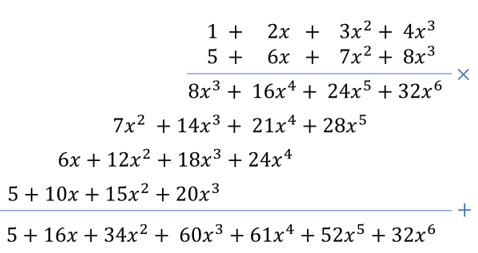
\includegraphics[width=0.6\textwidth]{./ntt_figures/1.png}
    \caption{Schoolbook method for polynomial multiplication or linear convolution with $O(n^2)$ complexity}
\end{figure}

\subsection{Cyclic Convolution}
Suppose that $G(x)$ and $H(x)$ are polynomials of degree $n-1$ in the quotient ring $\frac{\mathbb{Z}_{q}[x]}{(x^{n}-1)}$ where $q \in \mathbb{Z}$. A cyclic convolution or positive wrapped convolution, $PWC(x)$ is defined as:

\[PWC(x) = \sum_{k=0}^{n-1} c_k x^k\]
where $c_{k}=\sum_{i=0}^{k}g_{i}h_{k-i}+\sum_{i=k+1}^{n-1}g_{i}h_{k+n-i} \mod q$. If $Y(x)$ is the result of their linear convolution in the ring $\mathbb{Z}_{q}[x]$, it also can be defined as:

\[PWC(x) = Y(x) \mod (x^n - 1)\]
Traditional or schoolbook methods to calculate a cyclic convolution through a polynomial multiplication are shown in Example 2.1, followed by a long division. \\ \\
\textbf{Example 2.2:} Let $G(x)=1+2x+3x^{2}+4x^{3}$ and $H(x)=5+6x+7x^{2}+8x^{3}$ or in vector notation: $g=[1,2,3,4],$ and $h=[5,6,7,8]$.
\begin{figure}[h]
\centering
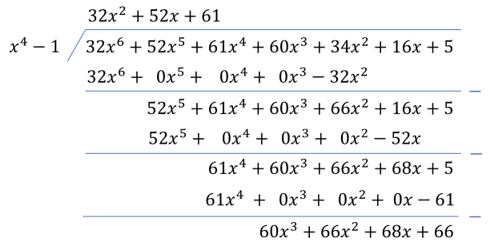
\includegraphics[width=0.6\textwidth]{./ntt_figures/2.png}
\caption{Schoolbook method for positively wrapped modular polynomial multiplication or cyclic convolution with $O(n^2)$ complexity}
\label{fig:cyclic_convolution}
\end{figure}

\noindent We have calculated $Y(x)$ in Example 2.1, thus we only need to do a long division by $x^{n}-1$

\subsection{Negacyclic Convolution}

Suppose that $G(x)$ and $H(x)$ are polynomials of degree $n-1$ in the quotient ring $\mathbb{Z}[x]/(x^{n}+1)$ where $q \in \mathbb{Z}$. A negacyclic convolution or negative wrapped convolution, $NWC(x)$ is defined as:

\[NWC(x) = \sum_{k=0}^{n-1} c_k x^k\]
where $c_{k}=\sum_{i=0}^{k}g_{i}h_{k-i}-\sum_{i=k+1}^{n-1}g_{i}h_{k+n-i} \mod q$. If $Y(x)$ is the result of their linear convolution in the ring $\mathbb{Z}[x]$, it also can be defined as

\[NWC(x) = Y(x) \mod (x^{n}+1)\] \\
\textbf{Example 2.3:} Let $G(x)=1+2x+3x^{2}+4x^{3}$ and $H(x)=5+6x+7x^{2}+8x^{3}$ or in vector notation: $g=[1,2,3,4]$ and $h=[5,6,7,8].$

\begin{figure}[H]
\centering
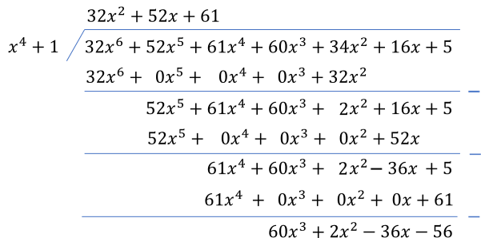
\includegraphics[width=0.6\textwidth]{./ntt_figures/3.png}
\caption{Schoolbook method for negatively wrapped modular polynomial multiplication or negacyclic convolution with $O(n^2)$ complexity}
\label{fig:negacyclic_convolution}
\end{figure}

\noindent We have calculated $Y(x)$ in Example 2.1, thus we only need to do a long division by $x^{n}+1$. \\ \\
Note that the only difference between cyclic and negacyclic convolution is the divisor. The cyclic convolution uses $x^n - 1$ while the negacyclic convolution uses $x^n + 1$. Those schoolbook algorithms have $O(n^2)$ complexity. Many efforts have been made to reduce their complexities by dividing the multiplier and multiplicand into several parts or by parallelizing the algorithm on the implementation side However, those efforts are not scalable as the polynomial degree grows higher.

\section{NTT-Based Convolution}
Many researchers do not differentiate the term NTT and FFT-based algorithms to calculate NTT, which creates confusion when understanding the topic. This report refers to the transformation itself as NTT and the FFT-like algorithms as fast-NTT. The classical NTT has a quadratic complexity of $O(n^2)$ when computed directly, while fast-NTT algorithms have a more efficient quasi-linear complexity $O(n \log n)$.

\subsection{Primitive $n^{th}$ Root of Unity}

Let $\mathbb{Z}_q$ be an integer ring modulo $q$, and $n-1$ is the polynomial degree of $G(x)$ and $H(x)$. Such rings have a multiplicative identity (unity) of 1. Define $\omega$ as a primitive $n$-th root of unity in $\mathbb{Z}_q$ if and only if:

\[\omega^n \equiv 1 \pmod{q}\]
and
\[\omega^k \not\equiv 1 \pmod{q}\]
for $k < n$.\\
One thing to note is that the primitive $n^{th}$ root of unity in a ring $\mathbb{Z}_q$ might not be unique. We show the following example for $q = 7681$ and $n = 4$. \\ \\
\textbf{Example 3.1:} In a ring $\mathbb{Z}_{7681}$ and $n = 4$, the 4-th roots of unity which satisfy the condition $\omega^4 \equiv 1 \pmod{7681}$ are $\{3383, 4298, 7680\}$. Out of three roots, $7680$ is not a primitive $n$-th root of unity, as there exist $k = 2 < n$ that satisfy $\omega^2 \equiv 1 \pmod{7681}$. Therefore $\omega = 3383$ or $\omega = 4298$ are the primitive 4-th roots of unity in $\mathbb{Z}_{7681}$.\\
\noindent The value of $\omega$ will be important in calculating NTT and positive wrapped convolution. Calculating the $\omega$ of a ring with a large number modulus $q$ is tricky and tedious.

\subsection{NTT-Based Positive-Wrapped Convolution}
This section explains the definition of Number Theoretic Transform (NTT) and its inverse (INTT) based on n-th root of unity, $omega$. The NTT of a polynomial does not have any physical meaning, unlike Discrete Fourier Transform (DFT) which represents a signal in the frequency domain. However, NTT preserves one of the important properties of DFT: the convolution theorem, which is valuable in calculating polynomial multiplication.

\subsubsection{Number Theoretic Transform Based on $\omega$}

The Number Theoretic Transform (NTT) of a vector of polynomial coefficients $a$ is defined as

\[\hat{a}_{j}=\sum_{i=0}^{n-1}\omega^{ij}a_{i} \mod q\]
where $j=0,1,2,...,n-1$.\\ \\
\textbf{Example 3.2:} Let $G(x)=1+2x+3x^{2}+4x^{3}$ or in vector notation $g=[1,2,3,4].$ We can infer that $n=4.$ Suppose we work in the ring $\mathbb{Z}_{7681}$ and $\omega$ is its primitive $n$-th root of unity. The NTT of $g$, $\hat{g}$, can be calculated by the following matrix multiplication:

\[\hat{g}=\begin{bmatrix}\omega^{0\times0}&\omega^{0\times1}&\omega^{0\times2}&\omega^{0\times3}\\ \omega^{1\times0}&\omega^{1\times1}&\omega^{1\times2}&\omega^{1\times3}\\ \omega^{2\times0}&\omega^{2\times1}&\omega^{2\times2}&\omega^{2\times3}\\ \omega^{3\times0}&\omega^{3\times1}&\omega^{3\times2}&\omega^{3\times3}\end{bmatrix}\begin{bmatrix}1\\ 2\\ 3\\ 4\end{bmatrix}\]
Notice that the power of $\omega$ is the multiplication between the row and column numbers. As $\omega$ is the $n$-root of unity, $\omega^{k}=\omega^{[k \mod n]}$ for $k>n.$ Thus:

\[\hat{g}=\begin{bmatrix}\omega^{0}&\omega^{0}&\omega^{0}&\omega^{0}\\ \omega^{0}&\omega^{1}&\omega^{2}&\omega^{3}\\ \omega^{0}&\omega^{2}&\omega^{4}&\omega^{6}\\ \omega^{0}&\omega^{3}&\omega^{6}&\omega^{9}\end{bmatrix}\begin{bmatrix}1\\ 2\\ 3\\ 4\end{bmatrix}\]

\[\hat{g}=\begin{bmatrix}\omega^{0}&\omega^{0}&\omega^{0}&\omega^{0}\\ \omega^{0}&\omega^{1}&\omega^{2}&\omega^{3}\\ \omega^{0}&\omega^{2}&\omega^{0}&\omega^{2}\\ \omega^{0}&\omega^{3}&\omega^{2}&\omega^{1}\end{bmatrix}\begin{bmatrix}1\\ 2\\ 3\\ 4\end{bmatrix}\]
From Example 3.1 we obtained one of the $n$-th roots of unity in $\mathbb{Z}_{7681}$ is $\omega=3383.$ Substituting into the equation:

\[\hat{g}=\begin{bmatrix}3383^{0}&3383^{0}&3383^{0}&3383^{0}\\ 3383^{0}&3383^{1}&3383^{2}&3383^{3}\\ 3383^{0}&3383^{2}&3383^{0}&3383^{2}\\ 3383^{0}&3383^{3}&3383^{2}&3383^{1}\end{bmatrix}\begin{bmatrix}1\\ 2\\ 3\\ 4\end{bmatrix}\]
\[\hat{g}=\begin{bmatrix}1&1&1&1\\ 1&3383&7680&4298\\ 1&7680&1&7680\\ 1&4298&7680&3383\end{bmatrix}\begin{bmatrix}1\\ 2\\ 3\\ 4\end{bmatrix}\]
\[\hat{g}=\begin{bmatrix}10\\ 913\\ 7679\\ 6764\end{bmatrix}\]
Therefore, the NTT($g$) = $[10,913,7679,6764]$ in $\mathbb{Z}_{7681}.$ \\ \\
\textbf{Example 3.3:} Let $H(x)=5+6x+7x^{2}+8x^{3}$ or in vector notation $h=[5,6,7,8]$ in the ring $\mathbb{Z}_{7681}$ and $\omega=3383.$ Using the same principle as Example 3.2, the NTT of $h$ is:

\[\hat{h}=\begin{bmatrix}1&1&1&1\\ 1&3383&7680&4298\\ 1&7680&1&7680\\ 1&4298&7680&3383\end{bmatrix}\begin{bmatrix}5\\ 6\\ 7\\ 8\end{bmatrix}=\begin{bmatrix}26\\ 913\\ 7679\\ 6764\end{bmatrix}\]
Therefore, the NTT($h$) = $[26,913,7679,6764]$ in $\mathbb{Z}_{7681}.$\\ \\
Note that the NTT of a particular polynomial is not always unique. It depends on the choice of $\omega$. The NTT result of Example 3.2 and 3.3 will differ if one uses $\omega=4298$ instead of $\omega=3383$.

\subsubsection{Inverse Number Theoretic Transform Based on $\omega$}

The Inverse of Number Theoretic Transform (INTT) of an NTT defined as

\[a_{i}=n^{-1}\sum_{j=0}^{n-1}\omega^{-ij}\hat{a}_{j} \mod q\]
and $j=0,1,2,...,n-1$.\\
Note that the INTT has a very similar formula to NTT. The only differences are $\omega$ replaced by its inverse in $\mathbb{Z}_q$ and a $n^{-1}$ scaling factor. It always holds that $a = \text{INTT}(\text{NTT}(a))$. \\ \\
\textbf{Example 3.4:} Given NTT($g$) = $\hat{g}$ = $[10,913,7679,6764]$ in $\mathbb{Z}_{7681}$ and $\omega=3383.$ We can calculate the inverse of $\omega$, which is $\omega^{-1}=4298$ and the scaling factor $n^{-1}=5761.$ One can calculate the INTT(NTT($g$)) by the following matrix multiplication:

\[g=n^{-1}\begin{bmatrix}\omega^{-0\times0}&\omega^{-0\times1}&\omega^{-0\times2}&\omega^{-0\times3}\\ \omega^{-1\times0}&\omega^{-1\times1}&\omega^{-1\times2}&\omega^{-1\times3}\\ \omega^{-2\times0}&\omega^{-2\times1}&\omega^{-2\times2}&\omega^{-2\times3}\\ \omega^{-3\times0}&\omega^{-3\times1}&\omega^{-3\times2}&\omega^{-3\times3}\end{bmatrix}\begin{bmatrix}10\\ 913\\ 7679\\ 6764\end{bmatrix}\]

\[g=n^{-1}\begin{bmatrix}\omega^{0}&\omega^{0}&\omega^{0}&\omega^{0}\\ \omega^{0}&\omega^{-1}&\omega^{-2}&\omega^{-3}\\ \omega^{0}&\omega^{-2}&\omega^{-4}&\omega^{-6}\\ \omega^{0}&\omega^{-3}&\omega^{-6}&\omega^{-9}\end{bmatrix}\begin{bmatrix}10\\ 913\\ 7679\\ 6764\end{bmatrix}\]

\[g=n^{-1}\begin{bmatrix}\omega^{0}&\omega^{0}&\omega^{0}&\omega^{0}\\ \omega^{0}&\omega^{-1}&\omega^{-2}&\omega^{-3}\\ \omega^{0}&\omega^{-2}&\omega^{0}&\omega^{-2}\\ \omega^{0}&\omega^{-3}&\omega^{-2}&\omega^{-1}\end{bmatrix}\begin{bmatrix}10\\ 913\\ 7679\\ 6764\end{bmatrix}\]

\[g=5761\begin{bmatrix}4298^{0}&4298^{0}&4298^{0}&4298^{0}\\ 4298^{0}&4298^{1}&4298^{2}&4298^{3}\\ 4298^{0}&4298^{2}&4298^{0}&4298^{2}\\ 4298^{0}&4298^{3}&4298^{2}&4298^{1}\end{bmatrix}\begin{bmatrix}10\\ 913\\ 7679\\ 6764\end{bmatrix}\]

\[g=5761\begin{bmatrix}1&1&1&1\\ 1&4298&7680&3383\\ 1&7680&1&7680\\ 1&3383&7680&4298\end{bmatrix}\begin{bmatrix}10\\ 913\\ 7679\\ 6764\end{bmatrix}=\begin{bmatrix}1\\ 2\\ 3\\ 4\end{bmatrix}\]
Therefore, the $g=[1,2,3,4],$ which is the initial polynomial coefficients given in Example 3.2 \\ \\
\textbf{Example 3.5:} 
Given NTT($h$) = $\hat{h}$ = $[26,913,7679,6764]$ in $\mathbb{Z}_{7681}$ and $\omega=3383.$ We can similarly calculate the INTT to the previous example:

\[
h = 5761 \begin{bmatrix}
1 & 1 & 1 & 1 \\
1 & 4298 & 7680 & 3383 \\
1 & 7680 & 1 & 7680 \\
1 & 3383 & 7680 & 4298
\end{bmatrix}
\begin{bmatrix}
26 \\
913 \\
7679 \\
6764
\end{bmatrix} = \begin{bmatrix}
5 \\
6 \\
7 \\
8
\end{bmatrix}
\]
Therefore, the $h=[5,6,7,8]$ which is the initial polynomial coefficients given in Example 3.3

\subsubsection{Using NTT to Calculate Positive-Wrapped Convolutions}
Because NTT is a variant of DFT in the polynomial ring. One can apply DFT's convolution theorem to calculate positive-wrapped convolution. \\
Let $a$ and $b$ are the multiplicands' vectors of polynomial coefficients. The positive-wrapped convolution of $a$ and $b$, $c$ can be calculated by:

\[c = \text{INTT}(\text{NTT}(a) \circ \text{NTT}(b))\]
where $\circ$ is an element-wise vector multiplication in $\mathbb{Z}_q$. \\ \\
\textbf{Example 3.6:} Let $g=[1,2,3,4]$ and $h=[5,6,7,8]$. From Example 3.2 and 3.3, we know that the NTT of them in $\mathbb{Z}_{7681}$ are $g^{\circ}=[10,913,7679,6764]$ and $\hat{h}=[26,913,7679,6764]$ when $\omega=3383.$ We can calculate their positive-wrapped convolution by:

\begin{align*}
    \text{INTT}\left(\begin{bmatrix}10\\913\\7679\\6764\end{bmatrix} \circ \begin{bmatrix}26\\913\\7679\\6764\end{bmatrix}\right) &= \text{INTT}\begin{bmatrix}260\\4021\\4\\3660\end{bmatrix} \\
    &= 5761 \begin{bmatrix}
    1 & 1 & 1 & 1 \\
    1 & 4298 & 7680 & 3383 \\
    1 & 7680 & 1 & 7680 \\
    1 & 3383 & 7680 & 4298
    \end{bmatrix}\begin{bmatrix}260\\4021\\4\\3660\end{bmatrix} = \begin{bmatrix}66\\68\\66\\60\end{bmatrix}
\end{align*}
Therefore, their positive-wrapped convolution is $[66,68,66,60]$, the same result as calculated by schoolbook multiplication and long division in Example 2.2.\\ \\
While positive-wrapped convolution, commonly known as cyclic convolution, is useful, its implementation is primarily outside the cryptography domain. However, in the context of PQC and HE, the chosen ring is mostly $\frac{\mathbb{Z}_{q}[x]}{(x^{n}+1)}$ instead of $\frac{\mathbb{Z}_{q}[x]}{(x^{n}-1)}$. One must calculate the polynomial multiplications via the negative-wrapped convolution in such rings.

\subsection{NTT-Based Negative-Wrapped Convolution}

This section explains the definition of Number Theoretic Transform (NTT) and its inverse (INTT) based on $2n$-th root of unity, $\psi$, and how to utilize them to calculate negative-wrapped or negacyclic convolution.

\subsubsection{Primitive $2n$-th Root of Unity}

To calculate negative-wrapped convolution, one needs the primitive $2n^{th}$ root of unity, $\psi$.\\ \\
Let $\mathbb{Z}_q$ be an integer ring modulo $q$, and $n-1$ is the polynomial degree of $G(x)$ and $H(x)$. $\omega$ is its primitive $n$-th root of unity. Define $\psi$ as the primitive $2n$-th root of unity if and only if:

\[\psi^{2} \equiv \omega \pmod{q} \quad \text{and} \quad \psi^{n} \equiv -1 \pmod{q}\]
\\
\textbf{Example 3.7:} In a ring $\mathbb{Z}_{7681}$ and $n=4$, when $\omega=3383$, the value of $\psi$ can be $1925$ or $5756$ as $1925^{2} \equiv 5756^{2} \equiv 3383 \pmod{7681}$ and $1925^{4} \equiv 5756^{4} \equiv 7680 \equiv -1 \pmod{7681}$. Therefore, one can choose the value $\psi=1925$ or $\psi=5756$.

\subsubsection{Number Theoretic Transform Based on $\psi$}

The Negative Wrapped Number Theoretic Transform (NTT) of a vector of polynomial coefficients $a$ is defined as $a^{\psi} = \text{NTT}^{\psi}\{a\}$, where:

\[\hat{a}_{j}=\sum_{i=0}^{n-1}\psi^{i}\omega^{ij}a_{i} \pmod{q}\]
and $j=0,1,2,...,n-1.$ As $\psi^{2} \equiv \omega \pmod{q}$, we can substitute $\omega$ to equation:

\[\hat{a}_{j}=\sum_{i=0}^{n-1}\psi^{2ij+i}a_{i} \pmod{q}\] \\
\textbf{Example 3.8:} Let $g=[1,2,3,4]$, $n=4$ and $\psi=1925$ in the ring $\mathbb{Z}_{7681}$. The NTT$^{\psi}(g) = \hat{g}$, can be calculated by the following matrix multiplication:

\[\hat{g}=\begin{bmatrix}\psi^{2(0\times0)+0}&\psi^{2(0\times1)+1}&\psi^{2(0\times2)+2}&\psi^{2(0\times3)+3}\\ \psi^{2(1\times0)+0}&\psi^{2(1\times1)+1}&\psi^{2(1\times2)+2}&\psi^{2(1\times3)+3}\\ \psi^{2(2\times0)+0}&\psi^{2(2\times1)+1}&\psi^{2(2\times2)+2}&\psi^{2(2\times3)+3}\\ \psi^{2(3\times0)+0}&\psi^{2(3\times1)+1}&\psi^{2(3\times2)+2}&\psi^{2(3\times3)+3}\end{bmatrix}\begin{bmatrix}1\\ 2\\ 3\\ 4\end{bmatrix}\]

\[\hat{g}=\begin{bmatrix}\psi^{0}&\psi^{1}&\psi^{2}&\psi^{3}\\ \psi^{0}&\psi^{3}&\psi^{6}&\psi^{9}\\ \psi^{0}&\psi^{5}&\psi^{10}&\psi^{15}\\ \psi^{0}&\psi^{7}&\psi^{14}&\psi^{21}\end{bmatrix}\begin{bmatrix}1\\ 2\\ 3\\ 4\end{bmatrix}\]

\[\hat{g}=\begin{bmatrix}1925^{0}&1925^{1}&1925^{2}&1925^{3}\\ 1925^{0}&1925^{3}&1925^{6}&1925^{9}\\ 1925^{0}&1925^{5}&1925^{10}&1925^{15}\\ 1925^{0}&1925^{7}&1925^{14}&1925^{21}\end{bmatrix}\begin{bmatrix}1\\ 2\\ 3\\ 4\end{bmatrix}\]

\[\hat{g}=\begin{bmatrix}1&1925&3383&6468\\ 1&6468&4298&1925\\ 1&5756&3383&1213\\ 1&1213&4298&5756\end{bmatrix}\begin{bmatrix}1\\ 2\\ 3\\ 4\end{bmatrix}\]

\[\hat{g}=\begin{bmatrix}1467\\ 2807\\ 3471\\ 7621\end{bmatrix}\]
Therefore, the NTT$^{\psi}(g)$ = $[1467,2807,3471,7621]$ when $\psi=1925$ in $\mathbb{Z}_{7681}$. \\ \\
\textbf{Example 3.9:} Let $h=[5,6,7,8]$, $n=4$ and $\psi=1925$ in the ring $\mathbb{Z}_{7681}$. The NTT$^{\psi}(h) = \hat{h}$, can be calculated similarly by the following matrix multiplication:

\[\hat{h}=\begin{bmatrix}1&1925&3383&6468\\ 1&6468&4298&1925\\ 1&5756&3383&1213\\ 1&1213&4298&5756\end{bmatrix}\begin{bmatrix}5\\ 6\\ 7\\ 8\end{bmatrix}=\begin{bmatrix}2489\\ 7489\\ 6478\\ 6607\end{bmatrix}\]
Therefore, the NTT$^{\psi}(h)$ = $[2489,7489,6478,6607]$.

\subsubsection{Inverse Number Theoretic Transform Based on $\psi$}

The Negative-Wrapped Inverse of Number Theoretic Transform (INTT) of an NTT vector $\hat{a}$ is defined as $a = \text{INTT}^{\psi}(\hat{a})$, where:
\[a_{i}=n^{-1}\sum_{j=0}^{n-1}\psi^{-j}\omega^{-ij}\hat{a}_{j} \pmod{q}\]
and $i=0,1,2,...,n-1.$ Substituting $\omega=\psi^{2}$ yields:
\[a_{i}=n^{-1}\sum_{j=0}^{n-1}\psi^{-(2ij+j)}\hat{a}_{j} \pmod{q}\] \\
Note that the differences between NTT and INTT are the scaling factor $n^{-1}$, the replacement of $\psi$ by $\psi^{-1}$, and the transpose of the exponents of the $\psi$ matrix.\\ \\
\textbf{Example 3.10:} Let NTT$^{\psi}(g)$ = $\hat{g}$ = $[1467,2807,3471,7621]$ and $\psi=1925$ in the ring $\mathbb{Z}_{7681}$. Note that $\psi^{-1}=1213$ and $n^{-1}=5761.$ The vector $g$ can be calculated by the following matrix multiplication:

\[g=n^{-1}\begin{bmatrix}\psi^{-0}&\psi^{-1}&\psi^{-2}&\psi^{-3}\\ \psi^{-0}&\psi^{-3}&\psi^{-6}&\psi^{-9}\\ \psi^{-0}&\psi^{-5}&\psi^{-10}&\psi^{-15}\\ \psi^{-0}&\psi^{-7}&\psi^{-14}&\psi^{-21}\end{bmatrix}\begin{bmatrix}1467\\ 2807\\ 3471\\ 7621\end{bmatrix}\]

\[g=n^{-1}\begin{bmatrix}\psi^{0}&\psi^{-1}&\psi^{-2}&\psi^{-3}\\ \psi^{0}&\psi^{-3}&\psi^{-2}&\psi^{-1}\\ \psi^{0}&\psi^{-2}&\psi^{0}&\psi^{-2}\\ \psi^{0}&\psi^{-1}&\psi^{-2}&\psi^{-3}\end{bmatrix}\begin{bmatrix}1467\\ 2807\\ 3471\\ 7621\end{bmatrix}\]

\[g=5761\begin{bmatrix}1213^{0}&1213^{1}&1213^{2}&1213^{3}\\ 1213^{0}&1213^{3}&1213^{6}&1213^{9}\\ 1213^{0}&1213^{5}&1213^{10}&1213^{15}\\ 1213^{0}&1213^{7}&1213^{14}&1213^{21}\end{bmatrix}\begin{bmatrix}1467\\ 2807\\ 3471\\ 7621\end{bmatrix}\]

\[g=5761\begin{bmatrix}1&1213&1467&1925\\ 1&1925&1467&1213\\ 1&1467&1&1467\\ 1&1213&1467&1925\end{bmatrix}\begin{bmatrix}1467\\ 2807\\ 3471\\ 7621\end{bmatrix}=\begin{bmatrix}1\\ 2\\ 3\\ 4\end{bmatrix}\]
Therefore $g=[1,2,3,4]$. \\ \\
\textbf{Example 3.11:} Let NTT$^{\psi}(h)$ = $\hat{h}$ = $[2489,7489,6478,6607]$ and $\psi = 1925$ in the ring $\mathbb{Z}_{7681}$. The vector $h$ can be calculated by the following matrix multiplication:

\[
h = 5761
\begin{bmatrix}
1 & 1 & 1 & 1 \\
1213 & 5756 & 6468 & 1925 \\
4298 & 3383 & 4298 & 3383 \\
5756 & 1213 & 1925 & 6468
\end{bmatrix}
\begin{bmatrix}
2489 \\
7489 \\
6478 \\
6607
\end{bmatrix} = \begin{bmatrix}
5 \\
6 \\
7 \\
8
\end{bmatrix}
\]
Therefore, the $h = [5,6,7,8]$.

\subsubsection{Using NTT$^{\psi}$ to Calculate Negative-Wrapped Convolutions}

Like its positive-wrapped version, the negative-wrapped NTT can evaluate the negative-wrapped convolutions, commonly referred to as negacyclic convolutions. \\ \\
Let $a$ and $b$ be the multiplicands' vectors of polynomial coefficients. The negative-wrapped convolution of $a$ and $b$, $c$ can be calculated by:

\[
c = \text{INTT}^{{\psi}^{-1}}(\text{NTT}^{\psi}(a) \circ \text{NTT}^{\psi}(b))
\] \\
\textbf{Example 3.12:} Let $g = [1,2,3,4]$ and $h = [5,6,7,8]$. From Example 3.8 and 3.9, we know that the NTT$^{\psi}$ of them in $\mathbb{Z}_{7681}$ are $\hat{g} = [1467,2807,3471,7621]$ and $\hat{h} = [2489,7489,6478,6607]$ when $\psi = 1925$. We can calculate their negative-wrapped convolution by:

\[
\text{INTT}^{\psi}\left(
\begin{bmatrix}
1467 \\
2807 \\
3471 \\
7621
\end{bmatrix}
\circ
\begin{bmatrix}
2489 \\
7489 \\
6478 \\
6607
\end{bmatrix}
\right) = \text{INTT}^{\psi}
\begin{bmatrix}
2888 \\
6407 \\
2851 \\
2992
\end{bmatrix}
\]

\[
= 5761
\begin{bmatrix}
1 & 1 & 1 & 1 \\
1213 & 5756 & 6468 & 1925 \\
4298 & 3383 & 4298 & 3383 \\
5756 & 1213 & 1925 & 6468
\end{bmatrix}
\begin{bmatrix}
2888 \\
6407 \\
2851 \\
2992
\end{bmatrix} =
\begin{bmatrix}
7625 \\
7645 \\
2 \\
60
\end{bmatrix}
\]
Therefore, $[7625,7645,2,60]$ or when written with negative numbers $[-56,-36,2,60]$ is their negacyclic convolution, the same result as calculated by schoolbook multiplication and long division in Example 2.3.

\section{Fast NTT}

In the previous sections, the presented NTT and INTT transformation pairs have $O(n^2)$ complexity, thus making no difference from the traditional method of negacyclic convolution. However, the NTT is the Discrete Fourier Transform in another ring. Therefore, the DFT optimization techniques can be applied to NTT. The well-known technique of DFT optimization is called the Fast-Fourier Transform (FFT), proposed independently by Cooley-Tukey and Gentleman-Sande. Both using similar butterflies divide-and-conquer technique to reduce the complexity to $O(n \log n)$.\\
To reduce the complexity and fasten the process of the matrix multiplication needed for the NTT transformation, one can use "divide and conquer" techniques by utilizing the periodicity and symmetry property of $\psi$:

\begin{align}
\text{periodicity} &: \psi^{k+2n} \equiv \psi^{k} \label{eq:periodicity} \\
\text{symmetry} &: \psi^{k+n} \equiv -\psi^{k} \label{eq:symmetry}
\end{align}
where $k$ is a non-negative integer. The calculation of a $n$ point NTT and INTT can be divided into two $n/2$ points. However, the dividing techniques for NTT and INTT are slightly different.

\subsection{Cooley-Tukey (CT) Algorithm for Fast-NTT}

\begin{align*}
    \hat{a}_{j} &= \sum_{i=0}^{n-1}\psi^{2ij+i}a_{i} \pmod{q} \\
    &= \sum_{i=0}^{n/2-1}\psi^{4ij+2i}a_{2i} + \sum_{i=0}^{n/2-1}\psi^{4ij+2j+2i+1}a_{2i+1} \pmod{q} \\
    &= \sum_{i=0}^{n/2-1}\psi^{4ij+2i}a_{2i} + \psi^{2j+1}\sum_{i=0}^{n/2-1}\psi^{4ij+2i}a_{2i+1} \pmod{q} \\
    \intertext{Based on the $\psi$'s symmetry properties:}
    \hat{a}_{j+n/2} &= \sum_{i=0}^{n/2-1}\psi^{4ij+2i}a_{2i} - \psi^{2j+1}\sum_{i=0}^{n/2-1}\psi^{4ij+2i}a_{2i+1} \pmod{q} \\
    \intertext{Let $A_{j}=\sum_{i=0}^{n/2-1}\psi^{4ij+2i}a_{2i}$ and $B_{j}=\sum_{i=0}^{n/2-1}\psi^{4ij+2i}a_{2i+1}$, equations become:}
    \hat{a}_{j} &= A_{j} + \psi^{2j+1}B_{j} \pmod{q} \\
    \hat{a}_{j+n/2} &= A_{j} - \psi^{2j+1}B_{j} \pmod{q}
    \end{align*}
Notice that $A_j$ and $B_j$ can be obtained as $n/2$ points NTT. If $n$ is power-of-two.
\begin{figure}[H]
    \centering
    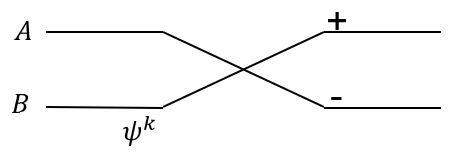
\includegraphics[width=0.5\textwidth]{./ntt_figures/4.png}
    \caption{Cooley-Tukey (CT) butterfly unit for calculating NTT}
    \label{fig:butterfly}
\end{figure}
\noindent One can configure several butterfly units to calculate the entire $n$ length of NTT. The idea is to calculate similar terms in the brackets once and then distribute the results instead of calculating them multiple times. The order of the results of CT-Butterfly is called bit-reversed order (BO), while the correct order of the NTT is called normal order (NO). \\ \\

\noindent \textbf{Example 3.13:} 
\[
\hat{g} = 
\begin{bmatrix}
\psi^0 & \psi^1 & \psi^2 & \psi^3 \\
\psi^0 & \psi^3 & \psi^6 & \psi^9 \\
\psi^0 & \psi^5 & \psi^{10} & \psi^{15} \\
\psi^0 & \psi^7 & \psi^{14} & \psi^{21}
\end{bmatrix}
\begin{bmatrix}
1 \\
2 \\
3 \\
4
\end{bmatrix}
\]

\begin{align*}
    g^0 &= 1\psi^0 + 2\psi^1 + 3\psi^2 + 4\psi^3 \\
    g^1 &= 1\psi^0 + 2\psi^3 + 3\psi^6 + 4\psi^9 \\
    g^2 &= 1\psi^0 + 2\psi^5 + 3\psi^{10} + 4\psi^{15} \\
    g^3 &= 1\psi^0 + 2\psi^7 + 3\psi^{14} + 4\psi^{21}
\end{align*}
Factoring:
\begin{align*}
    g'_0 &= \psi^0(1 + 3\psi^2) + \psi^1(2 + 4\psi^2) \\
    g'_1 &= \psi^0(1 + 3\psi^6) + \psi^3(2 + 4\psi^6) \\
    g'_2 &= \psi^0(1 + 3\psi^{10}) + \psi^5(2 + 4\psi^{10}) \\
    g'_3 &= \psi^0(1 + 3\psi^{14}) + \psi^7(2 + 4\psi^{14}) \\
\end{align*}
Based on the $\psi$ periodicity:
\begin{align*}
    g'_0 &= \psi^0(1 + 3\psi^2) + \psi^1(2 + 4\psi^2) \\
    g'_1 &= \psi^0(1 + 3\psi^6) + \psi^3(2 + 4\psi^6) \\
    g'_2 &= \psi^0(1 + 3\psi^2) + \psi^5(2 + 4\psi^2) \\
    g'_3 &= \psi^0(1 + 3\psi^6) + \psi^7(2 + 4\psi^6) 
\end{align*}
Based on the $\psi$ symmetry:
\begin{align*}
    g'_0 &= \psi^0(1 + 3\psi^2) + \psi^1(2 + 4\psi^2) \\
    g'_1 &= \psi^0(1 - 3\psi^2) + \psi^3(2 - 4\psi^2) \\
    g'_2 &= \psi^0(1 + 3\psi^2) - \psi^1(2 + 4\psi^2) \\
    g'_3 &= \psi^0(1 - 3\psi^2) - \psi^3(2 - 4\psi^2)
\end{align*}
\begin{figure}[H]
    \centering
    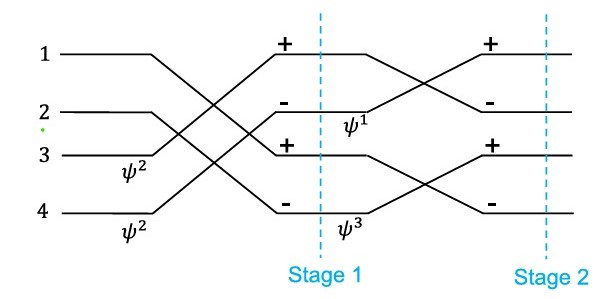
\includegraphics[width=0.7\textwidth]{./ntt_figures/5.jpg}
    \caption{CT Butterflies for n = 4 and [1, 2, 3, 4] as its input}
\end{figure}


\subsection{Gentleman-Sande (GS) Algorithm for Fast-INTT}

To calculate INTT, one will need another but similar "divide and conquer" approach.\\
For the INTT, instead of dividing the summation by its index parity, it is separated by the lower and upper half of the summation. From equation (16) and ignoring $n^{-1}$ term:

\begin{align*}
a_{i} &= \sum_{j=0}^{n-1}\psi^{-(2i+1)j}\hat{a}_{j} \pmod{q} \\
&= \left[\sum_{j=0}^{\frac{n}{2}-1}\psi^{-(2i+1)j}\hat{a}_{j}+\sum_{j=0}^{\frac{n}{2}-1}\psi^{-(2i+1)(j+\frac{n}{2})}\hat{a}_{(j+\frac{n}{2})}\right] \pmod{q} \\
&=\psi^{-i}\left[\sum_{j=0}^{\frac{n}{2}-1}\psi^{-2ij}\hat{a}_{j}+\sum_{j=0}^{\frac{n}{2}-1}\psi^{-2i(j+\frac{n}{2})}\hat{a}_{(j+\frac{n}{2})}\right] \pmod{q}
\end{align*}
Based on the periodicity and symmetry of $\psi^{-1}$, for the even term:
\begin{align*}
a_{2i} &= \psi^{-2i}\left[\sum_{j=0}^{\frac{n}{2}-1}\psi^{-4ij}\hat{a}_{j}+\sum_{j=0}^{\frac{n}{2}-1}\psi^{-4i(j+\frac{n}{2})}\hat{a}_{(j+\frac{n}{2})}\right] \pmod{q} \\
a_{2i} &= \psi^{-2i}\sum_{j=0}^{\frac{n}{2}-1}\left[\hat{a}_{j}+\hat{a}_{(j+\frac{n}{2})}\right]\psi^{-4ij} \pmod{q}
\end{align*}
Doing the same derivation for the odd term:
\[a_{2i+1}=\psi^{-2i}\sum_{j=0}^{\frac{n}{2}-1}\left[\hat{a}_{j}-\hat{a}_{(j+\frac{n}{2})}\right]\psi^{-4ij} \pmod{q}\]

Let $A_{i}=\sum_{j=0}^{\frac{n}{2}-1}\hat{a}_{j}\psi^{-4ij}$ and $B_{i}=\sum_{j=0}^{\frac{n}{2}-1}\hat{a}_{j+\frac{n}{2}}\psi^{-4ij},$
\begin{align*}
a_{2i} &= (A_i + B_i)\psi^{-2i} \pmod{q} \\
a_{2i+1} &= (A_i - B_i)\psi^{-2i} \pmod{q}
\end{align*}
Notice that $A_i$ and $B_i$ can be obtained as $\frac{n}{2}$ points INTT.
\begin{figure}[H]
    \centering
    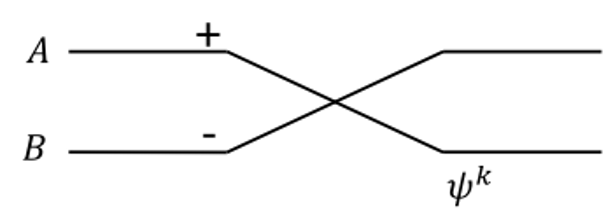
\includegraphics[width=0.5\textwidth]{./ntt_figures/6.png}
    \caption{Gentleman-Sande (GS) butterfly unit for calculating INTT}
\end{figure}
\textbf{Example 3.14:}
\begin{align*}
    g &= n^{-1} \begin{bmatrix}
    \psi^{-0} & \psi^{-0} & \psi^{-0} & \psi^{-0} \\
    \psi^{-1} & \psi^{-3} & \psi^{-5} & \psi^{-7} \\
    \psi^{-2} & \psi^{-6} & \psi^{-10} & \psi^{-14} \\
    \psi^{-3} & \psi^{-9} & \psi^{-15} & \psi^{-21}
    \end{bmatrix}
    \begin{bmatrix}
    1467 \\ 2807 \\ 3471 \\ 7621
    \end{bmatrix}
\end{align*}
\begin{align*}
    g_0 &= n^{-1}(1467\psi^{-0} + 2807\psi^{-0} + 3471\psi^{-0} + 7621\psi^{-0}) \\
    g_1 &= n^{-1}(1467\psi^{-1} + 2807\psi^{-3} + 3471\psi^{-5} + 7621\psi^{-7}) \\
    g_2 &= n^{-1}(1467\psi^{-2} + 2807\psi^{-6} + 3471\psi^{-10} + 7621\psi^{-14}) \\
    g_3 &= n^{-1}(1467\psi^{-3} + 2807\psi^{-9} + 3471\psi^{-15} + 7621\psi^{-21})
\end{align*}
Factoring:
\begin{align*}
    g_0 &= n^{-1}(\psi^{-0}(1467 + 3471) + \psi^{-0}(2807 + 7621)) \\
    g_1 &= n^{-1}(\psi^{-1}(1467 + 3471\psi^{-4}) + \psi^{-3}(2807 + 7621\psi^{-4})) \\
    g_2 &= n^{-1}(\psi^{-2}(1467 + 3471\psi^{-8}) + \psi^{-6}(2807 + 7621\psi^{-8})) \\
    g_3 &= n^{-1}(\psi^{-3}(1467 + 3471\psi^{-12}) + \psi^{-9}(2807 + 7621\psi^{-12}))
\end{align*}
Based on the $\psi$ periodicity:
\begin{align*}
    g_0 &= n^{-1}(\psi^{-0}(1467 + 3471) + \psi^{-0}(2807 + 7621)) \\
    g_1 &= n^{-1}(\psi^{-1}(1467 + 3471\psi^{-4}) + \psi^{-3}(2807 + 7621\psi^{-4})) \\
    g_2 &= n^{-1}(\psi^{-2}(1467 + 3471\psi^{0}) + \psi^{-5}(2807 + 7621\psi^{0})) \\
    g_3 &= n^{-1}(\psi^{-3}(1467 + 3471\psi^{4}) + \psi^{-1}(2807 + 7621\psi^{4})) 
\end{align*}
Based on the $\psi$ symmetry:
\begin{align*}
    g_0 &= n^{-1}(\psi^{-0}(1467 + 3471) + \psi^{-0}(2807 + 7621)) \\
    &= \psi^{-0}(\psi^{-0}(1467 + 3471) + \psi^{-0}(2807 + 7621)) \\
    g_1 &= n^{-1}(\psi^{-1}(1467 - 3471\psi^{0}) + \psi^{-3}(2807 - 7621\psi^{0})) \\ &= \psi^{-0}(\psi^{-1}(1467 - 3471\psi^{0}) + \psi^{-3}(2807 - 7621\psi^{0})) \\
    g_2 &= n^{-1}(\psi^{-2}(1467 + 3471\psi^{0}) - \psi^{-2}(2807 + 7621\psi^{0})) \\ &= \psi^{-2}((1467 + 3471\psi^{0}) - (2807 + 7621\psi^{0})) \\
    g_3 &= n^{-1}(\psi^{-3}(1467 - 3471\psi^{0}) + \psi^{-1}(2807 - 7621\psi^{0})) \\ &= \psi^{-2}(\psi^{-1}(1467 - 3471\psi^{0}) - \psi^{-3}(2807 - 7621\psi^{0}))
\end{align*}
\begin{figure}[H]
    \centering
    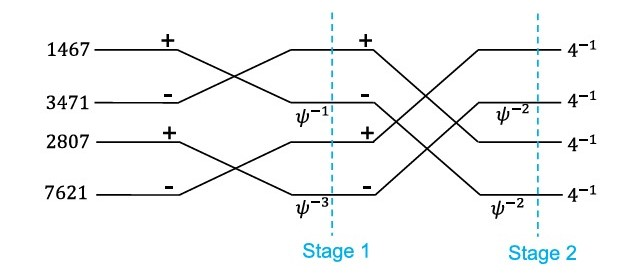
\includegraphics[width=0.7\textwidth]{./ntt_figures/7.jpg}
    \caption{GS Butterflies for n = 4 and [1467, 2807, 3471, 7621] as its input}
\end{figure}

\chapter{RISC-V}

RISC-V is a modern, open-source Instruction Set Architecture (ISA) that has gained significant traction in academia and industry for its simplicity, modularity, and flexibility. Unlike proprietary ISAs, RISC-V is freely available under a permissive license, enabling researchers and engineers to use, modify, and extend the architecture without incurring licensing costs or restrictions. This open nature makes it particularly attractive for developing hardware accelerators and custom systems tailored to specific applications.

\section{Overview of RISC-V Architecture}
RISC-V follows the Reduced Instruction Set Computing (RISC) principles, which emphasize simplicity and efficiency in instruction design. It provides a base integer instruction set (RV32I or RV64I) that includes essential operations, while optional extensions, such as floating-point (F), atomic (A), and vector (V) instructions, allow developers to adapt the ISA to different workloads. This modularity ensures that systems can be designed with only the necessary features, minimizing hardware complexity and power consumption.\\
The adoption of RISC-V offers several key advantages over traditional ISAs:
\begin{itemize}
    \item \textbf{Open-Source Flexibility}: RISC-V's open-source nature allows unrestricted access to the ISA specifications, fostering innovation and collaboration among researchers and companies.
    \item \textbf{Customizability}: Unlike fixed ISAs, RISC-V enables developers to add custom instructions and extensions to suit specific workloads, improving performance for specialized tasks.
    \item \textbf{Scalability}: RISC-V supports designs ranging from simple microcontrollers to high-performance processors, making it versatile for a wide range of applications.
    \item \textbf{Ecosystem and Toolchain}: RISC-V has a growing ecosystem, including compilers, simulators, and hardware development tools, which simplifies the development of custom systems.
\end{itemize}

\section{RISC-V Registers}

RISC-V architecture defines a set of general-purpose registers (GPRs) that are used for storing data and addresses during program execution. The base integer ISA (RV32I or RV64I) includes 32 GPRs, labeled x0 to x31, where x0 is hardwired to zero and serves as the constant zero register. The remaining registers are used for general-purpose computation and data manipulation.

\section{Instruction Fields}

RISC-V instructions are composed of several fields, each serving a specific purpose. These fields define the operation to be performed, the source and destination registers, and any immediate values required for the instruction. Table \ref{tab:instruction_fields_detail} provides an overview of these fields and their roles.

\begin{table}[H]
    \centering
    \caption{RISC-V Instruction Fields}
    \label{tab:instruction_fields_detail}
    \begin{tabular}{|>{\centering\arraybackslash}m{0.12\textwidth}|>{\centering\arraybackslash}m{0.12\textwidth}|>{\raggedright\arraybackslash}m{0.6\textwidth}|} % Adjusted widths
        \hline
        \textbf{Field} & \textbf{Bit Width} & \textbf{Purpose} \\
        \hline
        \texttt{Opcode} & 7 & Specifies the operation type and determines the instruction format. \\
        \hline
        \texttt{rd} & 5 & Destination register that stores the result of the operation. \\
        \hline
        \texttt{funct3} & 3 & Encodes the operation's sub-type within the opcode. It refines the instruction's functionality. \\
        \hline
        \texttt{rs1} & 5 & First source register used in the operation. \\
        \hline
        \texttt{rs2} & 5 & Second source register used in two-operand operations. \\
        \hline
        \texttt{funct7} & 7 & Provides additional differentiation for the instruction, particularly for operations like shifts and arithmetic. \\
        \hline
        \texttt{Immediate} & Variable & Encodes constants or offsets required for specific instructions. Immediate values are always sign-extended. \\
        \hline
    \end{tabular}
\end{table}


\section{Base ISA}

The RISC-V base ISA includes four primary instruction formats (R, I, S, U) and two additional formats (B, J) for handling different types of immediates. All base instructions are 32 bits in length and must be aligned to a four-byte boundary in memory. Misalignment exceptions are triggered for taken branches or jumps targeting non-aligned addresses. Extensions, such as compressed instructions, allow for two-byte alignment by reducing instruction lengths to 16 bits. Key aspects include:
\begin{itemize}
    \item Immediate values are sign-extended for simplicity and efficient hardware implementation.
    \item Register fields (rs1, rs2, rd) are fixed across formats to reduce decoding complexity.
    \item Immediate fields vary across formats but are packed and aligned to reduce hardware complexity and maintain efficient sign extension.
\end{itemize}

\begin{figure}[H]
    \centering
    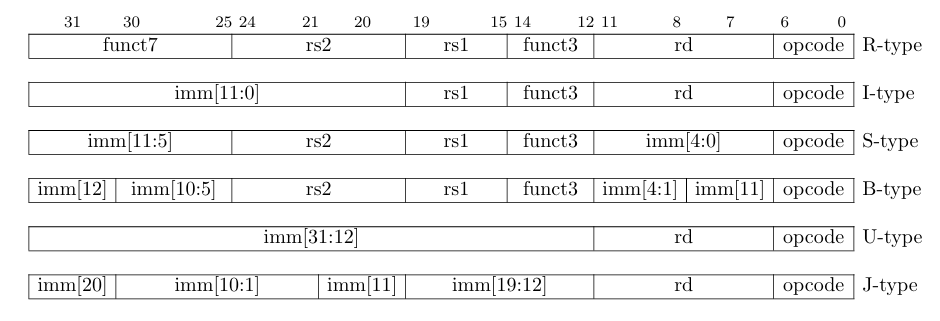
\includegraphics[width=1\textwidth]{./figures/riscv-base-isa.png}
    \caption{RISC-V Base Instruction Formats}
\end{figure}

Instruction formats serve different purposes:

\begin{itemize}
    \item \textbf{R-Type}: Used for register-register operations, where two source registers are specified along with a destination register.
    \item \textbf{I-Type}: Used for immediate operations, where one source register is combined with an immediate value to produce a result.
    \item \textbf{S-Type}: Used for store operations, where a source register is stored in memory using an immediate offset.
    \item \textbf{U-Type}: Used for upper immediate operations, where an immediate value is loaded into a register.
    \item \textbf{B-Type}: Used for branch operations, where two source registers are compared, and a branch is taken based on the result.
\end{itemize}

\chapter{Vortex GPGPU}

The Vortex GPGPU is a RISC-V-based GPU architecture designed for high-throughput parallel processing of data-parallel workloads. It features a SIMT execution model, where multiple threads execute the same instruction stream in lockstep, enabling efficient processing of vectorized computations.

\section{SIMD \& SIMT Execution}

\subsection{SIMD}  
Single Instruction, Multiple Data (SIMD) enables a single instruction to operate on multiple data elements simultaneously, ideal for vectorized computations with regular data patterns. It is widely used in GPUs and multimedia units for accelerating parallelizable workloads. 

\subsection{SIMT}  
Single Instruction, Multiple Threads (SIMT) is a GPU execution model where multiple threads execute the same instruction path concurrently, processing independent data elements. It efficiently handles data-parallel workloads by leveraging the GPU's thread-level parallelism. Each 32 or 64 threads are grouped into a \textbf{warp}, which executes the same instruction in lockstep. This model allows for divergence in thread execution, where threads can follow different paths but still execute the same instruction stream.

\begin{table}[H]
    \centering
    \caption{Key Differences Between SIMD and SIMT}
    \begin{tabular}{|>{\centering\arraybackslash}m{0.2\textwidth}|>{\centering\arraybackslash}m{0.35\textwidth}|>{\centering\arraybackslash}m{0.35\textwidth}|}
        \hline 
        \textbf{Aspect} & \textbf{SIMD} & \textbf{SIMT} \\
        \hline
        \textbf{Execution Unit} & Operates on multiple data elements with a single instruction & Operates multiple threads in parallel on different data \\
        \hline
        \textbf{Independence} & All data elements must follow the same operation (1 PC) & Threads can diverge but still execute the same instruction stream (Multiple PCs) \\
        \hline
    \end{tabular}
    \label{tab:simd_vs_simt}
\end{table}

\begin{figure}[H]
    \centering
    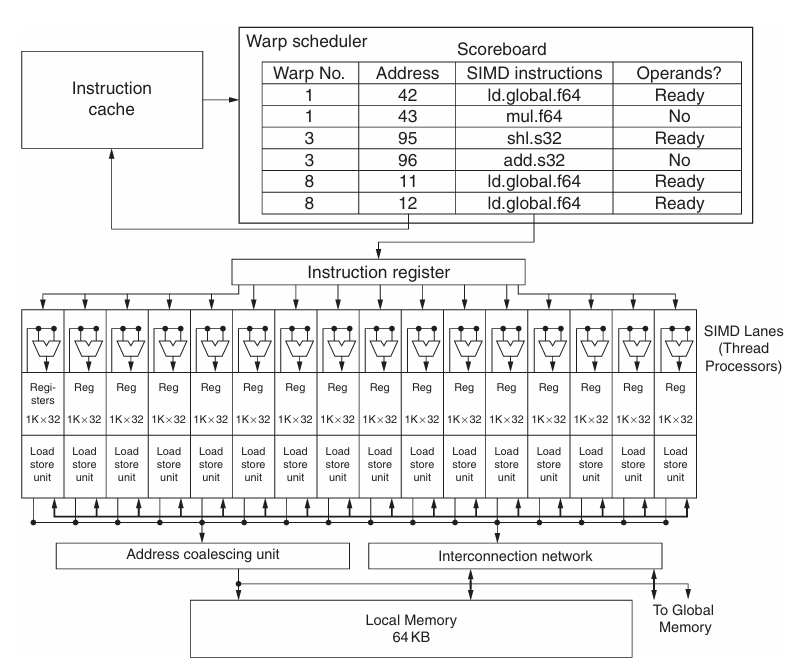
\includegraphics[width=1\textwidth]{./figures/simt.png}
    \caption{Simplified block diagram of a Multithreaded SIMD Processor}
\end{figure}

\section{Microarchitecture}

The vortex microarchitecture is a hierarchical design designed to maximize data throughput and minimize latency by leveraging parallelism at multiple levels.

\begin{itemize}
    \item \textbf{Processor}: The entire processing unit, which contains groups of cluster sharing L3 cache.
    \item \textbf{Cluster}: A group of sockets that share L2 cache.
    \item \textbf{Socket}: A physical unit that contains multiple cores and share L1 cache.
    \item \textbf{Core}: An individual processing unit within a socket, which contains the execution pipeline.
\end{itemize}

\begin{figure}[H]
    \centering
    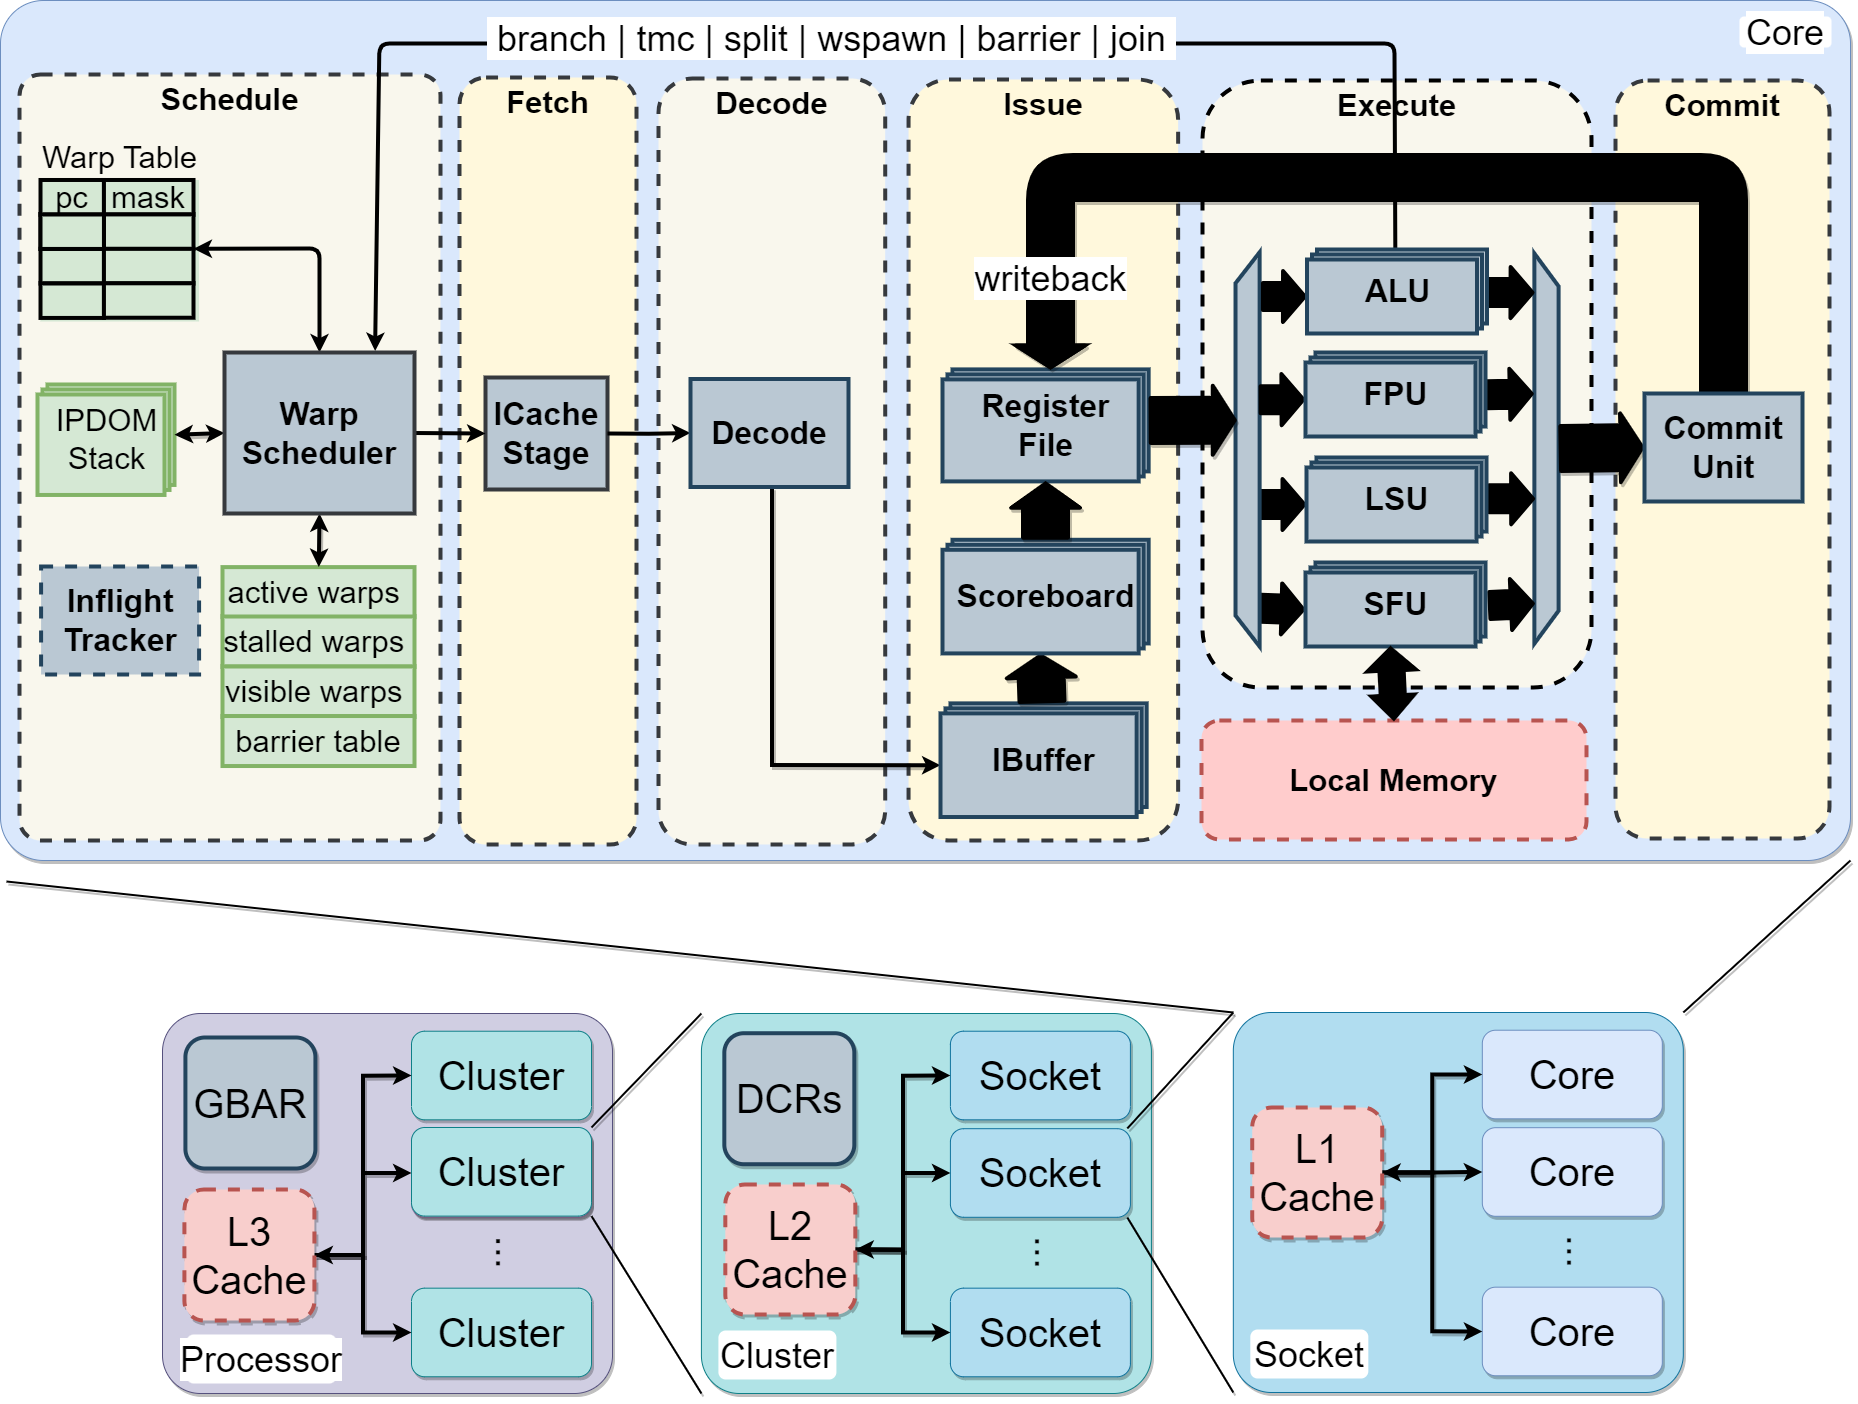
\includegraphics[width=1\textwidth]{./figures/vortex_microarchitecture.png}
    \caption{Vortex Microarchitecture}
\end{figure}

\section{Core Pipeline}

The core pipeline consists of 6 stages, each responsible for a specific operation in the instruction execution process. Pipelining helps improve throughput by allowing multiple instructions to be processed simultaneously.

\subsection{Schedule Stage}

The Schedule Stage is the initial stage in the pipeline, playing a pivotal role in the execution of warps. It ensures the smooth progression of instructions through the pipeline by carefully selecting and managing warps. key responsiblities include:
\begin{itemize}
    \item \textbf{Warp Selection:} Chooses a warp to propagate to subsequent stages in the pipeline, prioritizing based on specific criteria such as readiness and resource availability.
    \item \textbf{Thread Mask Management:} Thread masks are used to track active threads within a warp, enabling efficient execution of instructions across multiple threads.
    \item \textbf{Program Counter (PC) Updates:} Adjusts the program counters (PC) of warps to point to the correct instruction for execution, ensuring accurate control flow.
    \item \textbf{Stall Handling:} Identifies and resolves stalls by unlocking warps that were previously blocked due to resource conflicts, dependencies, or other pipeline constraints.
\end{itemize}
The schedule stage operates as follows:
\begin{itemize}
    \item Using the signals from warp control unit in the execute stage, new warps are spawned using \texttt{WSPAWN} instruction, so the schdule stage updates the active warps tracker.
    \item Schedule stage updates the active thread masks using branch divergence instructions like \texttt{JOIN} \& \texttt{SPLIT} as well as barrier synchronization instructions like \texttt{BAR} are handled.
    \item The schedule stage also updates the program counter (PC) when encountering branch instructions like \texttt{BRANCH} or \texttt{JUMP}.
    \item The schedule stage updates the CSR with information like number of cycles, the active warps, and thread masks.
    \item A leading zero counter selects the the warp to be scheduled from the active warps.
\end{itemize}
\begin{figure}[H]
    \centering
    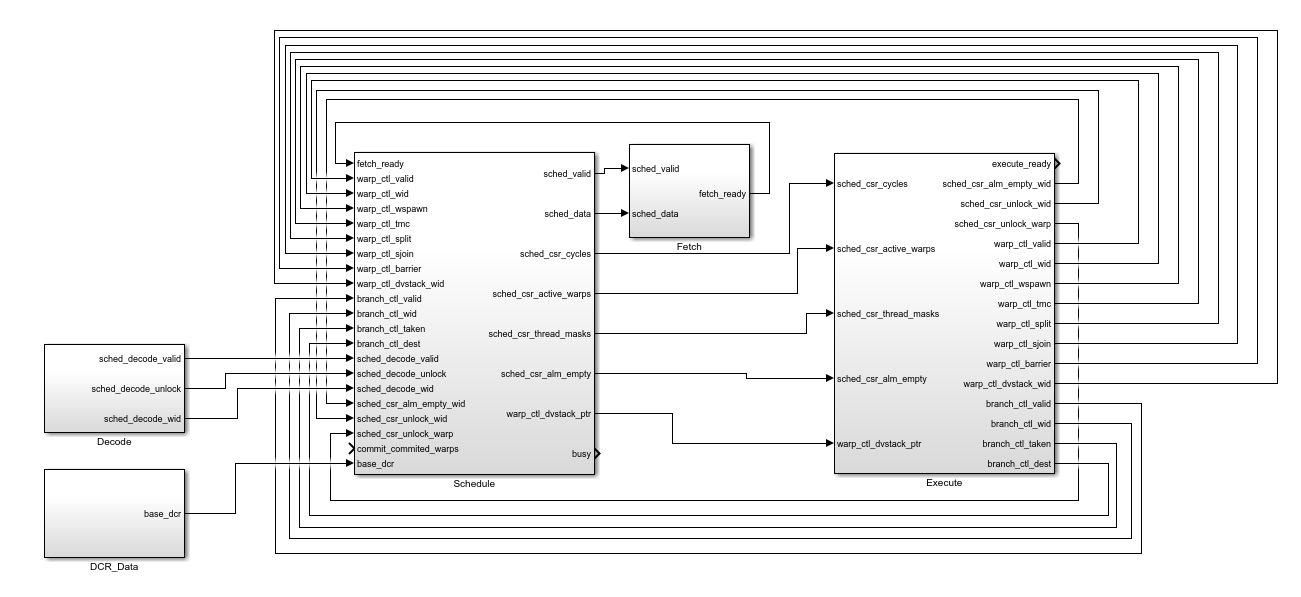
\includegraphics[width=0.8\textwidth]{./figures/schedule.png}
    \caption{Block Diagram of the Schedule Stage}
\end{figure}

\subsection{Fetch Stage}
The Fetch Stage is responsible for retrieving instructions from the instruction cache, ensuring that the correct instructions are delivered to the pipeline for active warps.  Key responsibilities include:
\begin{itemize}
    \item \textbf{Instruction Fetching:} Requests instructions from the instruction cache (Icache) based on the Program Counter (PC) provided by the schedule stage.
    \item \textbf{Warp Context Management:} Maintains context information such as thread masks and PCs for each warp to ensure accurate handling of instruction data.
\end{itemize}
Fetch stage prevents deadlocks in case of cacheless memory access with the help of signals from issue stage indicating that the instruction buffer is not full yet.
\begin{figure}[H]
    \centering
    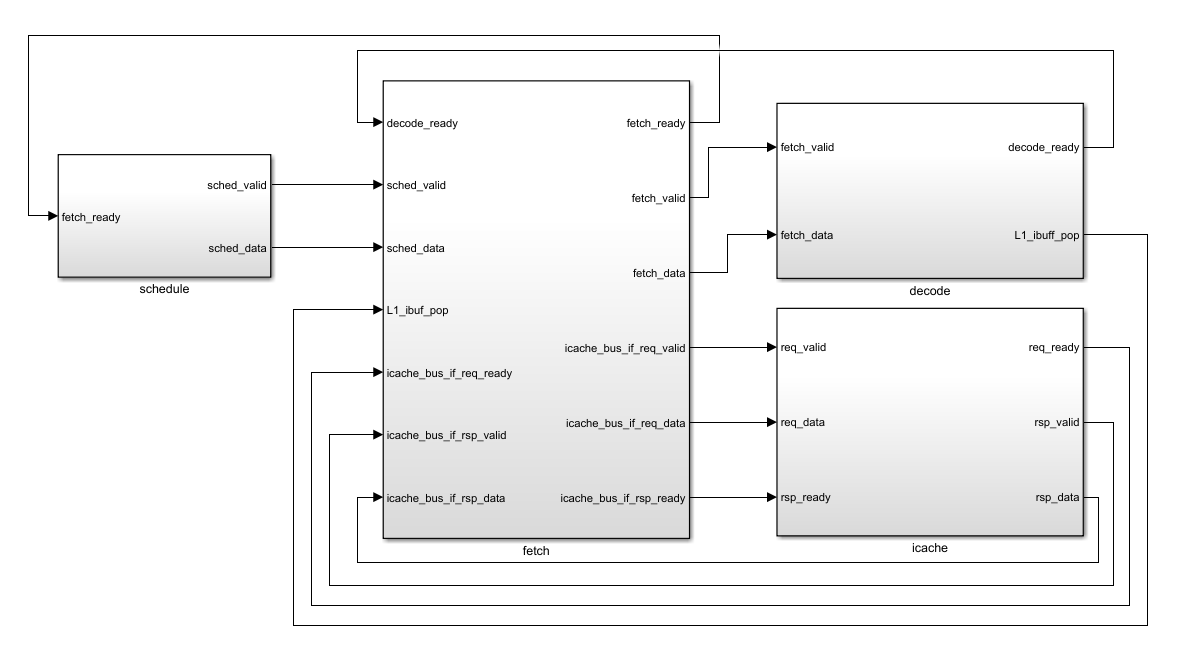
\includegraphics[width=0.8\textwidth]{./figures/fetch.png}
    \caption{Block Diagram of the Fetch Stage}
\end{figure}


\subsection{Decode Stage}
The Decode Stage is responsible for decoding fetched instructions and preparing them for execution. It extracts relevant information from the instruction stream, such as operation type, register operands, and immediate values, to facilitate efficient processing. The instruction is broken down to:
\begin{itemize}
    \item \textbf{Operation Type:} Determines the type of operation to be performed (e.g., arithmetic, load/store, branch).
    \item \textbf{Register Operands:} Identifies the source and destination registers for the instruction.
    \item \textbf{Operand Arguments:} Extracts immediate values or offsets and other flags or control bits required for the instruction.
    \item \textbf{Execution Type:} Specifies the execution unit or functional unit required to execute the instruction.
    \item \textbf{Writeback Flag:} Indicates whether the instruction result should be written back to the register file.
\end{itemize}
\begin{figure}[H]
    \centering
    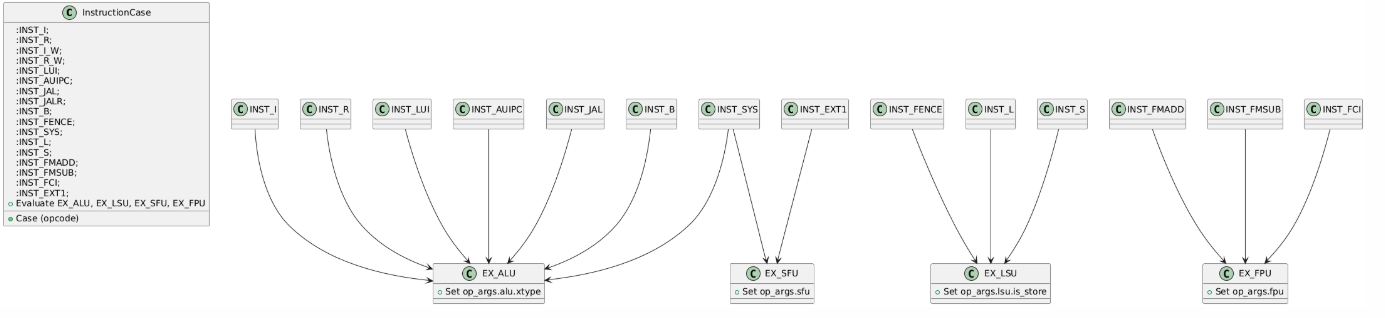
\includegraphics[width=1\textwidth]{./figures/decode2.png}
    \caption{Mapping of different instruction types to different execution units}
\end{figure}

\begin{figure}[H]
    \centering
    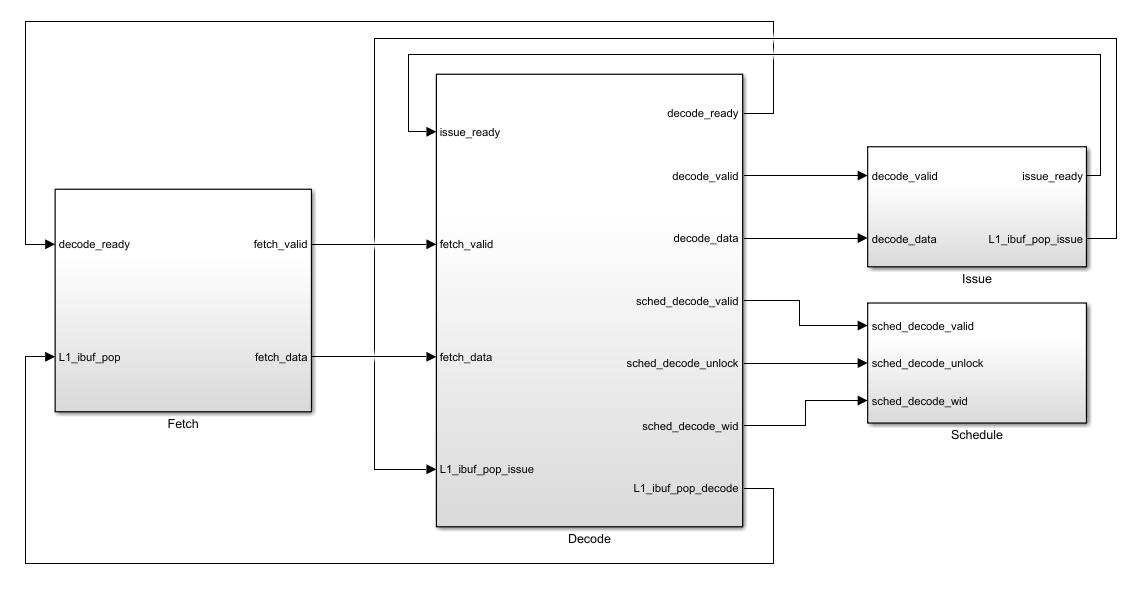
\includegraphics[width=0.8\textwidth]{./figures/decode.png}
    \caption{Block Diagram of the Decode Stage}
\end{figure}

\subsection{Issue Stage}
The Issue Stage introduces a second and third scheduling mechanism to efficiently manage instruction dependencies while optimizing data access. These mechanisms work to ensure that instructions are issued in an order that minimizes stalls and maximizes parallelism, enhancing overall performance. Additionally, they aim to maximize bank hits during data fetching, reducing memory access latency and improving throughput. Key responsibilities include:
\begin{itemize}
    \item \textbf{Instruction Buffer Management:} Stores multiple instructions fetched from memory to prevent stalling when there is a dependency.
    \item \textbf{Dependency Tracking:} Utilizes the scoreboard to identify and manage data and structural hazards between instructions, ensuring that issued instructions do not introduce pipeline hazards. This tracking allows overlapping the execution of instructions within the same warp.
    \item \textbf{Operand Access Optimization:} Relies on the operand collector to increase parallelism by maximizing register bank hits. This reduces access contention and improves throughput for source operands during instruction execution.
\end{itemize}
\begin{figure}[H]
    \centering
    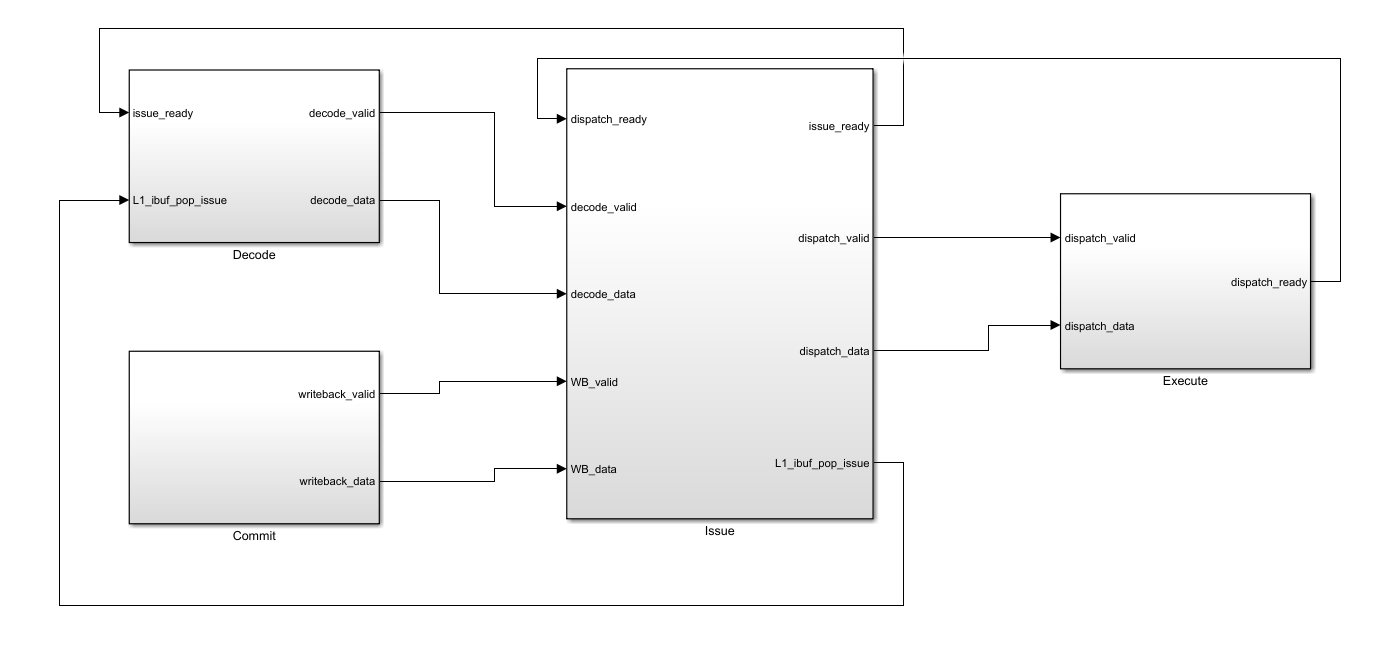
\includegraphics[width=0.7\textwidth]{./figures/issue_top.png}
    \caption{Block Diagram of the Issue Stage}
\end{figure}
\noindent The total number of warps is divided into slices, where each slice is equal to 8 warps and share the following:

\subsubsection{Instruction Buffer}
The instruction buffer is a FIFO (First-In, First-Out) structure that holds multiple decoded instructions, allowing multiple instruction to be stored in case if the instruction will cause hazards. This helps improve the flow of instructions through the pipeline. The instruction buffer also helps reduce delays caused by instruction cache misses by working with instruction miss-status holding registers (MSHRs), making sure that memory delays don't slow down the pipeline too much.

\subsubsection{Scoreboard}
The scoreboard manages data dependencies between instructions in a GPU core. It uses a simple in-order design to track the readiness of operands and registers for each warp. When an instruction enters the instruction buffer, the scoreboard is accessed to check for dependencies between operands and previously issued instructions. If dependencies are detected, the instruction is stalled until the required operands are available. This design prevents:

\begin{itemize}
    \item \textbf{RAW hazards:} They are prevented by checking if an instruction is trying to read a register that is currently being written to by a previous instruction. If the register is being written, the instruction will be stalled until the write completes.
    \item \textbf{WAW hazards:} They are avoided by ensuring that two instructions do not write to the same register simultaneously. The scoreboard tracks which instructions are writing to each register and stalls any subsequent instructions that attempt to write to the same register before the previous write is completed.
\end{itemize}

\subsubsection{Operand Collector}
The operand collector retrieves source operands for instructions from the instruction buffer by interacting with the scoreboard and general-purpose registers (GPRs). It ensures that operands are fetched only when their data is ready, preventing unnecessary delays. To support parallel accesses, the collector uses a multi-bank GPR design and incorporates arbitration to resolve bank conflicts. Each source operand is connected to each register file bank by a crossbar connection. The bank access is pipelined as shown in the figure below.
\begin{figure}[H]
    \centering
    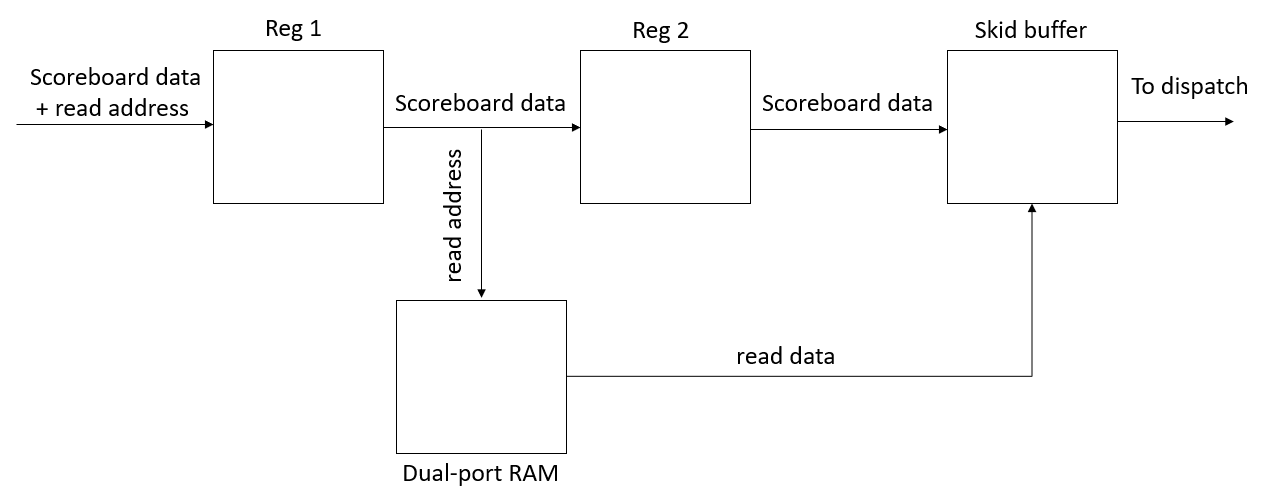
\includegraphics[width=0.7\textwidth]{./figures/operand_collector.png}
    \caption{Block Diagram of Operand Collector}
\end{figure}

\subsubsection{Dispatch}
It is responsible for dispatching operands to execution units in a GPU pipeline. It interfaces with the operand collector to fetch data and ensures that operands are ready before forwarding them to the appropriate execution unit. Each execution unit has an associated skid buffer, which temporarily holds operands to resolve pipeline hazards and maintain a steady flow of data.

\begin{figure}[H]
    \centering
    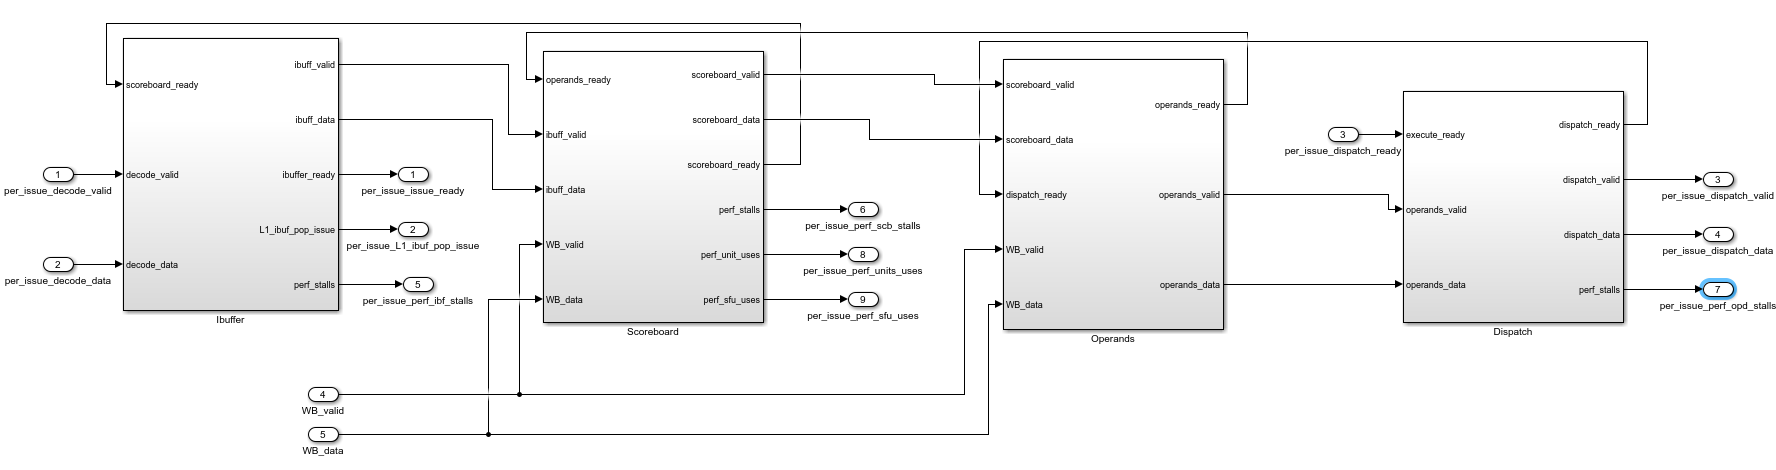
\includegraphics[width=01\textwidth]{./figures/issue_slice.png}
    \caption{Block Diagram of Issue Slice}
\end{figure}

\subsection{Execute Stage} \label{execute}
Execute stage is responsible for managing instruction execution in a GPU architecture. It integrates multiple execution units, including ALU, LSU, SFU, and optionally, FPU. Each unit interacts with its respective dispatch, commit, and memory interfaces, as well as the overall control logic. Key responsibilities include:
\begin{itemize}
    \item \textbf{Dispatch:} Dispatches the data of each thread to the appropriate execution unit based on the instruction type. It supports configurable block sizes, lane counts, and output buffering to handle diverse workloads.
    \item \textbf{Gather:} Recombines each thread data from the execution units into a single output, ensuring that the results are correctly aligned and formatted for further processing.
    \item \textbf{Local Memory Access:} Manages data access to the local memory, including load/store operations and data transfers between the execution units and memory banks.
\end{itemize}

\subsubsection{Dispatch Unit}
Recall that 1 issue slice is equal to 8 warps, and each warp has 32 threads. In 1 clock cycle, only 1 warp is selected, but due to stalling, we can have multiple warps executing in parallel in the same cycle if the warps are from different issue slices. Each issue slices is connected to an execution block, and the number of execution blocks is configurable.
\begin{itemize}
    \item \textbf{Batch Dispatch Logic} \\
    If the number of issue slices is greater than the number of blocks, the slices are divided to batches. The unit uses an arbiter to select the next batch of valid dispatch instructions. The selected batch index is updated on each cycle. It keeps track of batch indices for dispatching instructions in a round-robin or priority-based manner.

    \item \textbf{Partial Thread Handling} \\
    If the number of threads is greater than the number of lanes, the unit splits threads into smaller groups (packets) based on the number of lanes. It handles the start (sop), end (eop), and intermediate packets for partially dispatched threads.

    \item \textbf{Data Routing} \\ 
    It maps dispatch instructions to the appropriate execution blocks based on the size of the block and batch index. It uses elastic buffers to synchronize data flow between the dispatch and execution stages.
\end{itemize}
\begin{figure}[H]
    \centering
    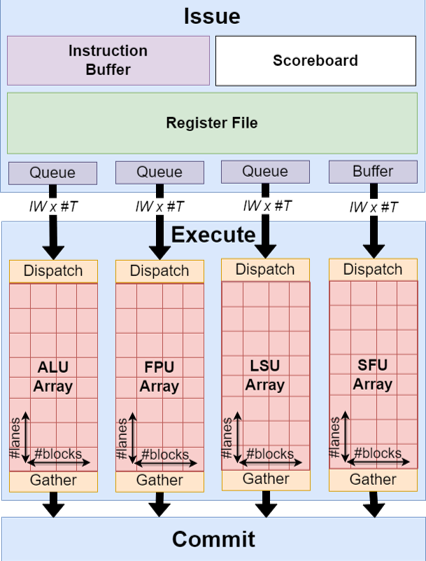
\includegraphics[width=0.5\textwidth]{./figures/dispatch.png}
    \caption{Dispatch and Gather of Threads}
\end{figure}
\subsubsection{ALU}

It handles the following:
\begin{itemize}
    \item \textbf{Arithmetic Operations:}
        \begin{itemize}
            \item Performs integer addition (\texttt{ADD}), subtraction (\texttt{SUB}), and comparison (\texttt{SLT, SLTU}).
            \item Supports wide and narrow operations (e.g., \texttt{ADDW, SUBW}).
        \end{itemize}

    \item \textbf{Logical Operations:}
        \begin{itemize}
            \item Implements logical operations such as AND, OR, XOR, and SLL (shift left logical).
            \item Supports sign-extension or zero-extension for operands based on the instruction type.
        \end{itemize}

    \item \textbf{Branch Operations:}
        \begin{itemize}
            \item Handles branch instructions by comparing results based on the operation type.
            \item Generates the branch destination address and determines whether the branch is taken or not.
        \end{itemize}
\end{itemize}

\subsubsection{FPU}
Floating Point Unit (FPU) is responsible for handling floating-point operations, including single-precision (32-bit) and double-precision (64-bit) arithmetic. It supports a wide range of operations, such as addition, subtraction, multiplication, division, and square root, ensuring accurate and efficient processing of floating-point data. It is optional and can be included based on the application requirements.

\subsubsection{SFU} 
Special Function Unit (SFU) contains:
\begin{itemize}
    \item \textbf{Warp Control Unit} \\
        Warp Control Unit is responsible for handling GPU custom instructions such as:
        \begin{itemize}
            \item \textbf{Branch Divergence/Convergence:} Threads in a warp move in a lockstep executing the same instruction. However, Branch Divergence happens when there is a condition on a certain thread within a warp so that each thread can follow different execution paths. The approach used is to serialize execution of threads following different paths within a given warp. To achieve this serialization of divergent code paths, a SIMT stack is used. Each entry on this stack contains three entries:
                \begin{itemize}
                    \item A reconvergence program counter (RPC)
                    \item The address of the next instruction to execute (Next PC)
                    \item An active mask
                \end{itemize}
                \begin{figure}[H]
                    \centering
                    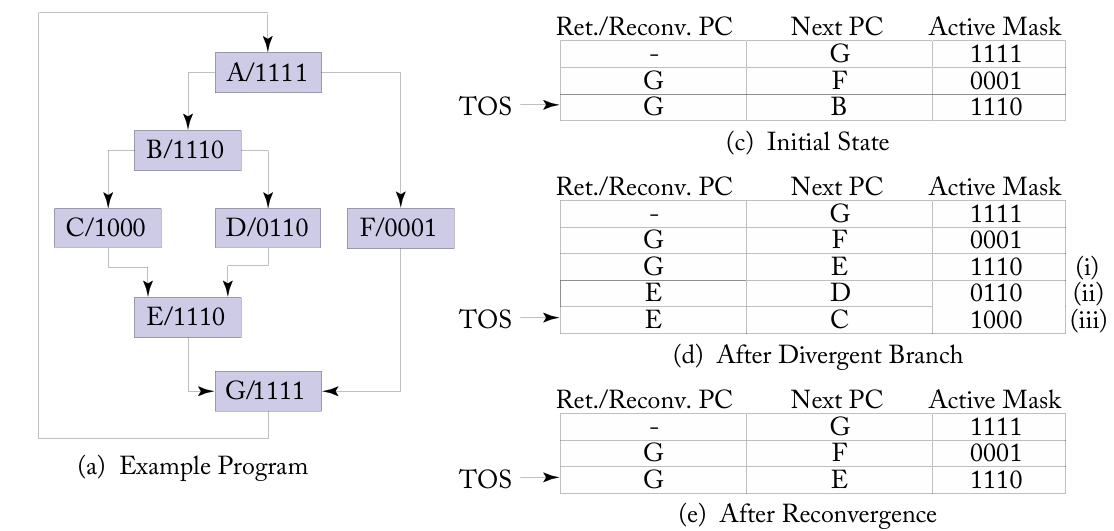
\includegraphics[width=0.8\textwidth]{./figures/simt-stack.png}
                    \caption{Branch Divergence and IPDOM Stack}
                \end{figure}
            \item \textbf{Barriers:} Branch divergence can potentially lead to deadlocks. When a branch divergence occurs, we must choose whether to execute the if or else path first. This can cause issues if there is a dependency between the statements inside the if block and those inside the else block. The solution is to alternate execution between the if and else statements. To ensure proper synchronization and avoid deadlocks, we introduce barriers at the reconvergence point, allowing warps to synchronize before proceeding.
                \begin{figure}[H]
                    \centering
                    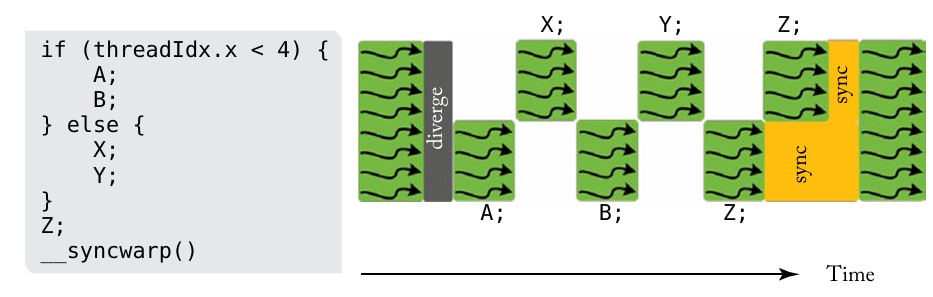
\includegraphics[width=0.7\textwidth]{./figures/barrier.png}
                    \caption{Barrier Handling in SIMT Execution}
                \end{figure}
            \item \textbf{TMC / PRED:} Responsible for thread mask control (based on a predicate or not). 
            \item \textbf{WSPAWN :} Responsible for spawning warps.
        \end{itemize}
    \item \textbf{CSR Unit}\\
    The CSR (Control and Status Register) unit is a critical component in RISC-V processors, responsible for managing various system-level and performance-related control registers. It handles the read and write operations for these registers, supporting architectural extensions such as floating-point operations. The CSR unit also facilitates interaction with performance counters, providing insights into metrics like active warps, thread masks, and memory performance. By enabling programmable control over processor behavior, it plays a vital role in both functional and performance aspects of the system.
\end{itemize}

\subsubsection{LSU}
The Load Store Unit (LSU)  is a critical module in GPU architectures designed for efficient memory management. It is responsible for handling memory operations, including loads, stores, and atomic operations, ensuring data integrity and maximizing memory throughput. Key responsibilities include:
\begin{itemize}
    \item \textbf{Address Calculation:} 
    Combines source operand data and an immediate offset to compute the full memory address for each active lane.
    
    \item \textbf{Byte Enable Handling:} 
    Dynamically generates byte-enable signals based on operation size (e.g., 8-bit, 16-bit, 32-bit, etc.).
    
    \item \textbf{Memory Scheduler Integration:} 
    Sends memory requests through the memory scheduler for optimized arbitration and access to memory channels.

    \item \textbf{Misaligned Access Detection:} 
    Asserts an error if an instruction attempts a misaligned memory access based on its operation size.
    
    \item \textbf{Response Formatting:} 
    Formats data from memory for each thread, applying alignment and sign-extension (or zero-extension) as needed.
\end{itemize}


\subsection{Memory Unit}
The memory unit is designed to handle a wide range of memory operations for GPUs. It manages memory interactions across local memory (LMEM) and data cache (DCACHE) while supporting multi-lane and multi-block configurations. The module ensures high performance through arbitration, coalescing, and efficient memory access strategies. Key responsibilities include:
\begin{itemize}
    \item \textbf{Local Memory Management (Optional)}
        \begin{itemize}
            \item Implements a local memory system for faster data access and reduced latency.
            \item Supports multi-bank memory architectures with configurable sizes and buffering.
        \end{itemize}
    \item \textbf{Data Cache Interaction}
        \begin{itemize}
            \item Interfaces with a data cache to handle global memory requests efficiently.
            \item Implements coalescing mechanisms to optimize memory traffic.
        \end{itemize}
    \item \textbf{Arbitration Between Memory Systems}
        \begin{itemize}
            \item Uses configurable arbitration schemes to prioritize requests between local and global memory.
            \item Includes switches and adapters for efficient communication.
        \end{itemize}
\end{itemize}

\subsubsection{Local Memory Switch}
The local memory switch module is a key component that arbitrates between global and local memory requests in a GPU's memory subsystem. This module ensures that memory requests are correctly routed to either local memory or global memory and handles responses accordingly.
\begin{itemize}
    \item Decides whether a memory request is intended for local or global memory. 
    \item Buffers requests and responses using elastic buffers to decouple the pipeline stages.
    \item Uses an arbiter to prioritize and merge memory responses from local and global memory.
\end{itemize}

\subsubsection{Memory Coalescer}
The memory coalescer module aggregates smaller memory requests into larger ones to optimize memory access patterns. It handles input requests and responses, coalesces them, and forwards them to the memory subsystem.
\begin{itemize}
    \item \textbf{Input Request Handling}
        \begin{itemize}
            \item The module accepts multiple parallel input requests, validates them, and identifies overlapping or coalescable requests based on their addresses. This reduces redundant requests to downstream memory units.
        \end{itemize}
    \item \textbf{Output Request Generation}
        \begin{itemize}
            \item Input requests are aggregated and merged to form larger output requests. Each output request represents multiple coalesced input requests, optimizing memory bandwidth.
        \end{itemize}
\end{itemize}

\subsubsection{Adapter}
The adapter (Dcache/Lmem) module bridges the LSU memory interface and the memory bus interface. It facilitates memory requests and responses across multiple lanes by packing and unpacking data streams efficiently.
\begin{itemize}
    \item \textbf{Unpacking Submodule}
        \begin{itemize}
            \item This submodule unpacks incoming LSU memory requests into individual lane-specific requests, distributing them across Number of Lanes.
        \end{itemize}
    \item \textbf{Packing Submodule}
        \begin{itemize}
            \item This submodule packs incoming memory responses from individual lanes into a single LSU memory response.
        \end{itemize}
\end{itemize}

\begin{figure}[H]
    \centering
    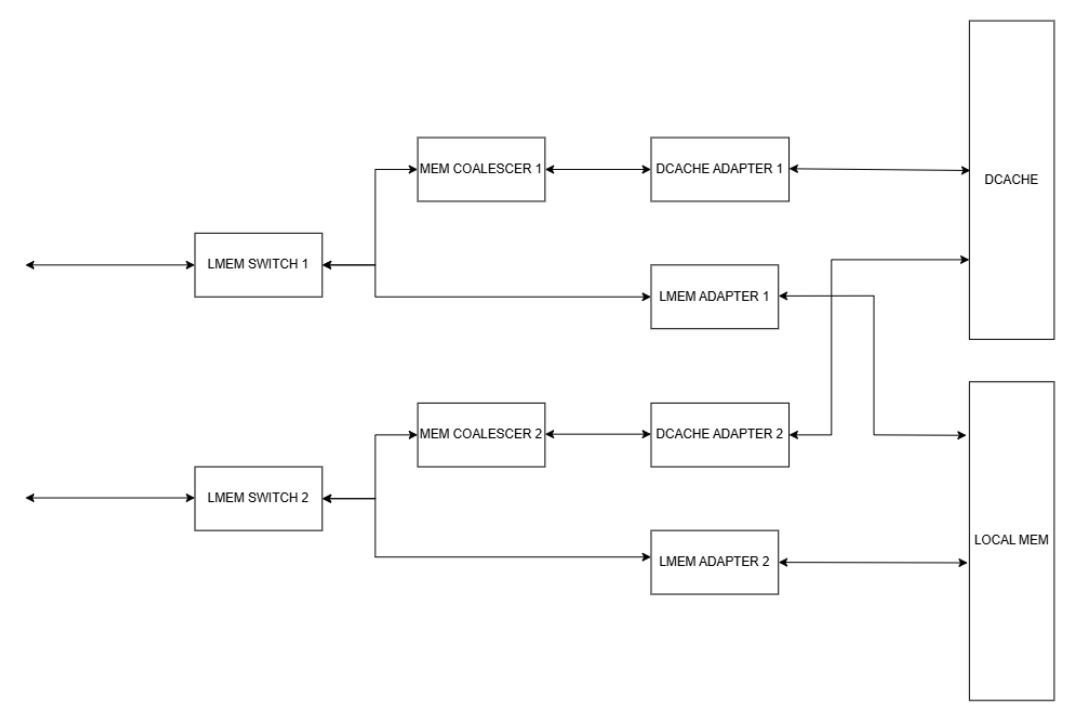
\includegraphics[width=0.7\textwidth]{./figures/mem_unit.png}
    \caption{Memory Unit Block Diagram}
\end{figure}

\begin{figure}[H]
    \centering
    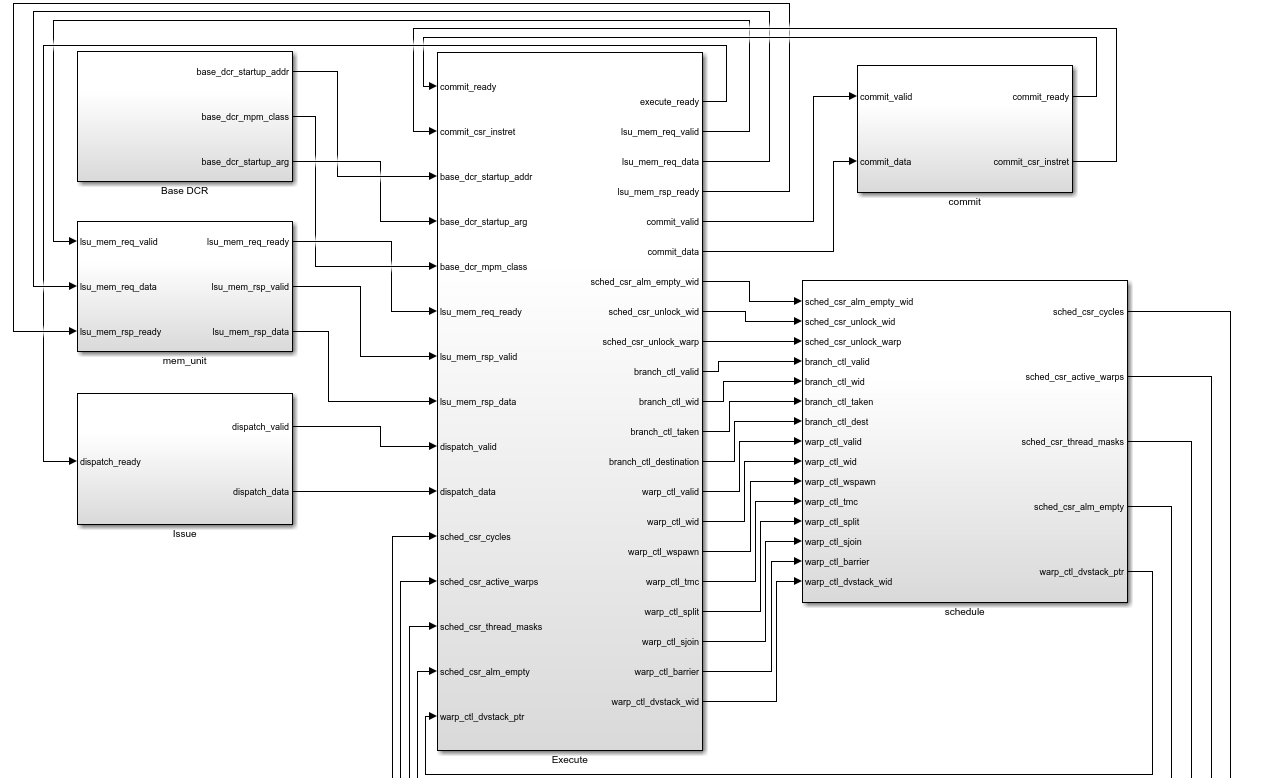
\includegraphics[width=1\textwidth]{./figures/execute.png}
    \caption{Block Diagram of the Execute Stage}
\end{figure}

\subsection{Commit Stage}

The Commit Stage is responsible for finalizing the execution of instructions, updating architectural state, and tracking performance metrics. It plays a crucial role in ensuring instructions are correctly retired and results are committed to the register file. Key responsibilities include:
\begin{itemize}
    \item \textbf{Arbitration and Prioritization:} Resolves contention among execution units by arbitrating between valid instructions from multiple sources.
    \item \textbf{Writeback Data Handling:} Manages the transfer of execution results to the register file in the issue stage.
    \item \textbf{Instruction Retirement:} Marks instructions as completed and retires them from the pipeline, and updates the CSR with such performance counters.
    \item \textbf{Warp Management:} Signals the schedule stage about completed warps, enabling efficient management of pipeline resources.
\end{itemize}

\begin{figure}[H]
    \centering
    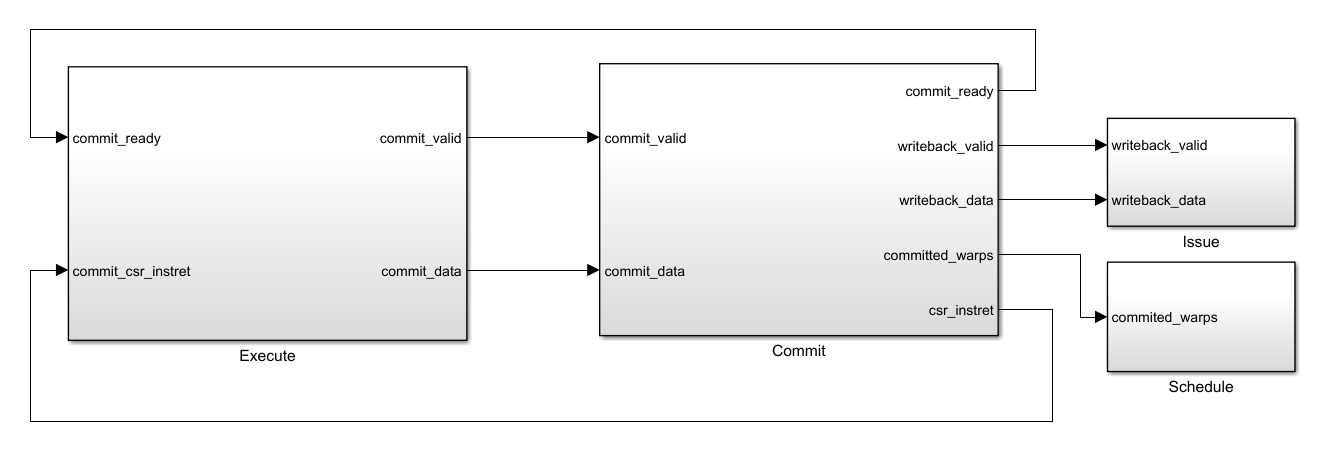
\includegraphics[width=0.8\textwidth]{./figures/commit.png}
    \caption{Block Diagram of the Commit Stage}
\end{figure}

\subsection{Interfaces between Stages}

\subsubsection{Handshake Protocol Using Skid Buffers}

Skid buffers are used to manage data flow between different stages. The handshake protocol ensures that data is transferred correctly and efficiently between these stages even when there is a downstream stage is stalled.

\begin{itemize}
    \item \textbf{Fire In}: When the upstream stage has valid data to send, it asserts the "Fire In" signal. This indicates that the data is ready to be stored in the skid buffer.
    
    \item \textbf{Store Data}: If the downstream stage is stalled (i.e., it cannot accept new data), the skid buffer temporarily stores the incoming data. This prevents data loss and allows the upstream stage to continue processing without waiting for the downstream stage to become ready.
    
    \item \textbf{Fire Out}: Once the downstream stage is ready to accept new data, the skid buffer asserts the "Fire Out" signal. This indicates that the stored data is now being forwarded to the downstream stage.
\end{itemize}
\begin{figure}[H]
    \centering
    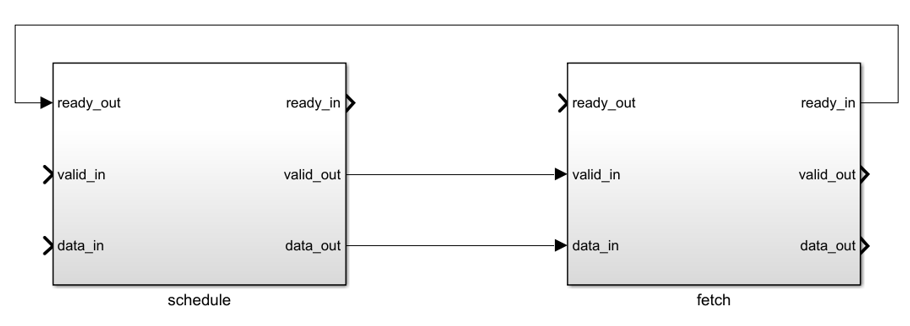
\includegraphics[width=0.8\textwidth]{./figures/handshake.png}
    \caption{Skid Buffer Handshake Protocol between Schedule \& Fetch Stages}
\end{figure}

\begin{table}[H]
\centering
\renewcommand{\arraystretch}{1.5} % Adjust row height
\begin{tabular}{|m{4cm}|m{11cm}|} \hline
\textbf{Stage} & \textbf{Output Data} \\\hline
Schedule Stage & PC, thread masks, warp ID \\\hline
Fetch Stage & Schedule data, instruction \\\hline
Decode & Schedule data, execution type, op type, op arguments, writeback flag, source and destination registers \\\hline
Issue & Schedule data, op type, op arguments, writeback flag, source and destination registers \\\hline
Execute & Schedule data, writeback flag, result, destination register, packet ID, eop, sop \\\hline
Commit & Schedule data, result, destination register, packet ID, eop, sop \\\hline
\end{tabular}
\caption{Data Propagation through the Pipeline Stages}
\label{tab:pipeline_stages}
\end{table}


\section{Software Stack}

The Vortex software stack is designed to facilitate the seamless execution of both host and GPU code, enabling efficient communication and task scheduling between the host and the Vortex GPGPU. The stack is divided into two main components: the host compilation flow and the GPU compilation flow. Each component plays a critical role in ensuring that the system can effectively manage memory operations, kernel launches, and hardware-specific optimizations.

\subsection{Host Compilation Flow}
The flow goes through the following steps:
\begin{enumerate}
    \item \textbf{Host Code Development:}
        \begin{itemize}
            \item Host code is written in C (.c files).
            \item The host code manages overall execution flow, memory operations (e.g., data transfers between host and device), and kernel launches (e.g., initiating GPU kernel execution).
        \end{itemize}
    \item \textbf{Host Compilation:}
        \begin{itemize}
            \item The host code is compiled using a standard C compiler (e.g., GCC, Clang).
            \item The compiler generates object files (.o files) from the .c files, and an executable file that interacts with the Vortex runtime library.
        \end{itemize}
    \item \textbf{Linking:}
        \begin{itemize}
            \item The object files are linked with the Vortex runtime library.
            \item The runtime library provides functions for memory management and kernel execution (e.g., \texttt{vx\_start} \& \texttt{vx\_copy\_to\_dev}).
        \end{itemize}
    \item \textbf{Executable Generation} 
\end{enumerate}
\begin{figure}[H]
    \centering
    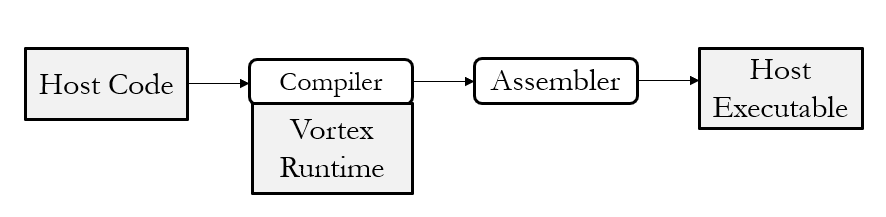
\includegraphics[width=0.8\textwidth]{./figures/host_comp.png}
    \caption{Host Compilation Flow}
\end{figure}

\subsection{GPU Compilation Flow}
The flow goes through the following steps:
\begin{enumerate}
    \item \textbf{Kernel Code Development:}
        \begin{itemize}
            \item Kernel code is written in OpenCL or CUDA.
        \end{itemize}
    \item \textbf{Front-end Compilation (PoCL):}
        \begin{itemize}
            \item The kernel code is processed by a front-end compiler.
            \item The front-end compiler generates Intermediate Representation (IR) from the kernel code, which can help improve optimization.
            \item Uses built-in libraries for math functions.
        \end{itemize}
    \item \textbf{Back-end Compilation (LLVM):}
        \begin{itemize}
            \item The IR is passed to a back-end compiler.
            \item The back-end compiler generates the kernel executable.
            \item Uses Vortex Kernel Library for accessing runtime information and controlling program flow (e.g., \texttt{vx\_spawn\_tasks} \& \texttt{vx\_num\_threads}).
            \item Uses Vortex ISA which inlcudes custom RISC-V instructions for the Vortex GPGPU.
        \end{itemize}
\end{enumerate}
\begin{figure}[H]
    \centering
    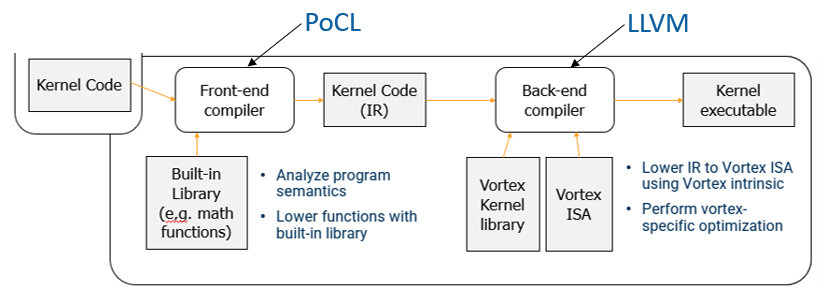
\includegraphics[width=0.8\textwidth]{./figures/gpu_comp.png}
    \caption{GPU Compilation Flow}
\end{figure}




\subsection{Vortex Execution flow}
The flow for the commands required for device communication, as outlined in the host code, adhere to the following execution sequence:
\begin{enumerate}
    \item \textbf{They are linked with the frontend runtime library.}
        \begin{itemize}
            \item The frontend runtime library outlines how frontend methods can be executed using the Vortex runtime library.
        \end{itemize}
    \item \textbf{The Vortex library carries out the operation using the Vortex host interface. 
}
        \begin{itemize}
            \item Vortex host interface, in turn, performs the operation on the Vortex processor, which is connected to the external bus via the Vortex host interface.
        \end{itemize}
\end{enumerate}
\begin{figure}[H]
    \centering
    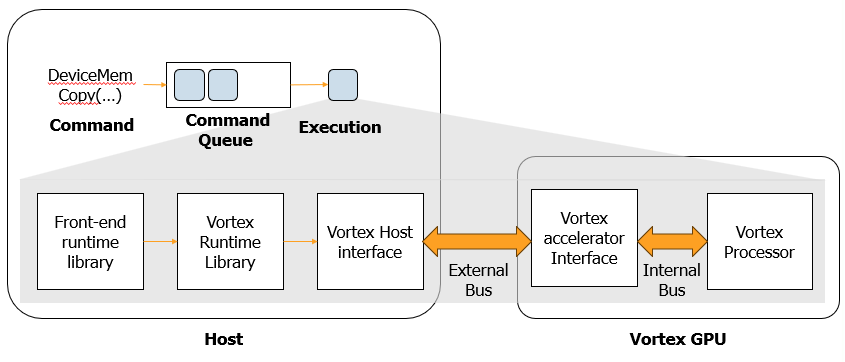
\includegraphics[width=0.8\textwidth]{./figures/execution_flow.png}
    \caption{Execution Flow}
\end{figure}



%\part{Methodology}

%\part{Implementation}

%\part{Results}

%\chapter{Conclusion}

\bibliographystyle{plain} % Choose a bibliography style
\bibliography{references} % Path to your .bib file (without the .bib extension)
\nocite{Satriawan2023}
\nocite{aamodt2018general}
\nocite{hennessy2011computer}
\nocite{vortex2023}


\end{document}

